%---------------------------------------------------------------------------------------------------------------------------- 
\graphicspath{{Parti/P04-Travi_rigide/P04-Travi_rigide/Figure/}}
\chapter{La trave rigida}\label{cap:Trave_Rigida}
%---------------------------------------------------------------------------------------------------------------------------- 

\begin{sommario}
	Si introduce la \emph{trave} come corpo rigido con
	una dimensione predominante --- la lunghezza ---
	rispetto alle dimensioni trasversali, dotata di un
	\emph{riferimento intrinseco} solidale alla linea
	d'asse e orientato univocamente dalla fibra inferiore.
	
	Si formulano il \emph{problema cinematico} e il
	\emph{problema statico} del vincolo di continuità
	interno: le grandezze duali sono le \emph{distorsioni}
	--- estensionale, trasversale e rotazionale --- e le
	\emph{caratteristiche della sollecitazione}, reazioni
	interne del vincolo di rigidità. Si introducono il
	\emph{metodo per equivalenza} per il calcolo delle
	caratteristiche lungo la trave, l'analisi del loro
	\emph{salto} nelle sezioni di singolarità e le
	\emph{equazioni indefinite di equilibrio} come forma
	differenziale dello stesso principio.
	
	Si mostra infine che il taglio ideale in una sezione
	interna lascia invariata la classificazione del
	sistema, e si distingue la \emph{trave monoconnessa},
	con caratteristiche determinate dal solo equilibrio,
	dalla \emph{trave pluriconnessa}, internamente
	iperstatica; si descrivono gli \emph{svincoli interni}
	che rilasciano parzialmente il vincolo di rigidità.
\end{sommario}



%----------------------------------------------------------------------------------------------------------------------------
\section{Definizione di trave}
\label{sec:trave_def}
%----------------------------------------------------------------------------------------------------------------------------


Si chiama \emph{trave}\index{trave|textbf}\index{trave!rigida|textbf} un corpo rigido la cui
geometria è caratterizzata da una dimensione
predominante, detta \emph{lunghezza}, rispetto
alle dimensioni trasversali. La trave è descritta
dalla sua \emph{linea d'asse}\index{linea d'asse|textbf} --- il luogo dei
baricentri delle \emph{sezioni trasversali} ---
che può essere rettilinea o curva. Si chiama
\emph{sezione trasversale}\index{sezione trasversale|textbf} in un punto $S$ della
linea d'asse il piano perpendicolare alla linea
d'asse in $S$; la sua intersezione con il corpo
è la \emph{sezione} della trave in $S$.
Se la linea d'asse giace in un piano si parla
di \emph{trave piana}\index{trave!piana|textbf}.



Il corpo reale è l'\emph{intorno tubolare} della
linea d'asse: le dimensioni trasversali $b$, $h$
sono piccole rispetto alla lunghezza $\ell$, e ai
fini dell'analisi cinematica e statica sono
irrilevanti.

Nell'ipotesi di rigidità, la forma della linea d'asse è
inessenziale per la cinematica e la statica: una trave
rigida piana è completamente descritta dai tre parametri
$(u(O), v(O), \vartheta)$ del suo polo, indipendentemente
dalla geometria della linea d'asse. Nelle figure si adotta
pertanto la convenzione di rappresentare ogni trave
mediante la sola linea d'asse, con i vincoli applicati
nei punti corrispondenti della linea d'asse, come
illustrato nella \FIGref{fig:trave_convenzione}.




\begin{oss}
	La definizione di trave non esclude corpi di forma
	più generale: un corpo rigido piano di forma
	qualsiasi può sempre essere trattato con gli stessi
	strumenti, semplicemente scegliendo un polo $O$
	conveniente. La specializzazione alla trave è una
	scelta di rappresentazione, non una limitazione
	della teoria. Essa è motivata dal fatto che nella
	pratica strutturale i corpi di interesse hanno quasi
	sempre geometria d'asse, e la rappresentazione
	tramite la linea d'asse semplifica considerevolmente
	la lettura delle figure.
\end{oss}

\begin{figure}[htbp]
	\centering
	\resizebox{\textwidth}{!}{%
		\begin{tikzpicture}[
			>=Stealth, line width=0.8pt, trave/.style={line width=1.5pt, line cap=round, line join=round, black},	terra/.style={line width=0.7pt, black},
			nodoV/.style={circle, fill=white, draw=black,	inner sep=0pt, minimum size=4pt}]
			
			% ================================================================
			% PANNELLO SINISTRO — trave reale
			% ================================================================
			\begin{scope}[xshift=0cm]
				
				\def\L{5.0}
				\def\H{0.70}
				\def\B{0.50}
				
				% corpo della trave: parallelepipedo prospettico
				% faccia frontale — aggiunto spigolo destro mancante
				\draw[thick] (0,0) rectangle (\L,\H);
				\draw[thick] (\L,0) -- (\L,\H);  % spigolo destro esplicito
				% spigolo verticale faccia destra posteriore
				\draw[thick] (\L+\B, \B) -- (\L+\B, \B+\H);
				
				
				% faccia frontale
				\draw[thick] (0,0) rectangle (\L,\H);
				% spigoli prospettici
				\draw[thick] (0,\H)  -- ++(\B,\B);
				\draw[thick] (\L,\H) -- ++(\B,\B);
				\draw[thick] (\L,0)  -- ++(\B,\B);
				% faccia superiore
				\draw[thick] (0,\H) -- ++(\B,\B)
				-- ++(\L,0)
				-- ++(-\B,-\B);
				% spigoli posteriori tratteggiati — DOPO la faccia frontale
				\draw[dashed,gray!60] (0,0)   -- ++(\B,\B);
				\draw[dashed,gray!60] (\B,\B) -- ++(\L,0);
				% spigolo verticale posteriore sinistro — per ultimo
				\draw[dashed,gray!60] (\B,\B) -- ++(0,\H);
				
				% linea d'asse: dal baricentro faccia sinistra
				\draw[trave] (\B/2, \H/2+\B/2) -- (\L+\B/2, \H/2+\B/2);
				\fill (\B/2, \H/2+\B/2) circle (2pt)	node[left=3pt]{\small$A$};
				\fill (\L+\B/2, \H/2+\B/2) circle (2pt)	node[right=3pt]{\small$B$};
				
				
				% quota h solo a sinistra
				\draw[|<->|,thin] (-0.35,0) -- (-0.35,\H)
				node[midway,left=2pt]{\small$h$};
				
				% quota b
				\draw[<->,thin] (\L+0.15,0)
				-- (\L+0.15+\B, \B)
				node[midway,right=1pt]{\small$b$};
				
				% quota L
				\draw[|<->|,thin] (0,-0.45) -- (\L,-0.45)
				node[midway,above=-1pt]{\small$\ell$};
				
				% etichetta pannello
				\node[below=20pt] at (\L/2, 0) {\small(a)};
				
			\end{scope}
			
			% ================================================================
			% PANNELLO DESTRO — schematizzazione
			% ================================================================
			
			\begin{scope}[xshift=7.5cm, yshift=0.6cm]
				
				\def\L{5.0}
				
				% linea d'asse
				\draw[trave] (0,0) -- (\L,0);
				
				
				% ferri di chiamata della quota (sotto i vincoli, grigi sottili)
				\draw[very thin, gray!50] (0,-0.85)  -- (0,-1.15);
				\draw[very thin, gray!50] (\L,-0.85) -- (\L,-1.15);
				
				
				% cerniera esterna in A (canone)
				\draw[terra] (0,0) -- ++(-0.22,-0.38)
				-- ++(0.44,0) -- cycle;
				\draw[terra] (-0.30,-0.38) -- (0.30,-0.38);
				\foreach \x in {-0.24,-0.12,0,0.12,0.24}
				\draw[very thin, black]
				(\x,-0.38) -- ++(-0.09,-0.11);
				\node[nodoV] at (0,0) {};
				\node[above=4pt] at (0,0) {$A$};
				
				% carrello esterno in B (canone, ridotto al 85%)
				\draw[terra] (\L,0) -- ++(-0.25,-0.36)
				-- ++(0.50,0) -- cycle;
				\draw[terra] (\L-0.34,-0.36) -- (\L+0.34,-0.36);
				\draw[terra] (\L-0.18,-0.50) circle (2.7pt);
				\draw[terra] (\L+0.18,-0.50) circle (2.7pt);
				\draw[terra] (\L-0.34,-0.64) -- (\L+0.34,-0.64);
				\foreach \x in {-0.28,-0.15,-0.02,0.11,0.24}
				\draw[very thin, black]
				(\L+\x,-0.64) -- ++(-0.10,-0.13);
				\node[nodoV] at (\L,0) {};
				\node[above=4pt] at (\L,0) {$B$};
				
				% quota L
				\draw[|<->|,thin] (0,-1.05) -- (\L,-1.05)
				node[midway,above=-1pt]{\small$\ell$};
				
				% etichetta pannello
				\node[below=35pt] at (\L/2, 0) {\small(b)};
				
				
			\end{scope}
			
		\end{tikzpicture}
	}
	\caption{Dalla trave reale alla schematizzazione
		strutturale.
		(a)~Trave reale: corpo rigido con
		lunghezza $\ell$ e dimensioni trasversali
		$b$, $h$ con $b,h \ll \ell$. La linea
		d'asse (tratteggiata spessa) è il luogo
		dei baricentri delle sezioni trasversali;
		gli estremi $A$ e $B$ sono i punti della
		linea d'asse corrispondenti alle facce
		terminali.
		(b)~Schematizzazione strutturale:
		si traccia la sola linea d'asse; i vincoli
		(cerniera in $A$, carrello in $B$) sono
		posizionati sui punti corrispondenti.
		Questa è la rappresentazione adottata in
		tutte le figure del capitolo.}
	\label{fig:trave_convenzione}
\end{figure}



%----------------------------------------------------------------------------------------------------------------------------
\subsection{Il riferimento intrinseco}
\label{sec:riferimento_intrinseco}
%----------------------------------------------------------------------------------------------------------------------------

A ciascuna trave si associa un \emph{riferimento
	intrinseco}\index{riferimento intrinseco|textbf}\nomenclature[L]{$(O^e;\,y^e,\,z^e)$}{riferimento intrinseco della trave} $(O^e;\, y^e,\, z^e)$. Nel seguito ci
limitiamo al caso della \emph{trave rettilinea piana},
con estremi $A$ e $B$: la linea d'asse è un segmento
nel piano, e il riferimento intrinseco è fisso lungo
tutta la trave. Il riferimento è definito come segue:

\begin{itemize}[nosep]
	\item l'asse $z^e$ è diretto lungo la linea d'asse,
	nel verso di percorrenza da $A$ a $B$;
	\item l'asse $y^e$ è nel piano della trave,
	perpendicolare a $z^e$, diretto verso la
	\emph{fibra inferiore}\index{fibra inferiore};
	\item l'asse $x^e$ è ortogonale al piano della
	trave, diretto in modo che il riferimento
	$(O^e;\, x^e, y^e, z^e)$ sia destrorso
	(asse $x^e$ uscente dal piano del foglio).
\end{itemize}

\begin{oss}
	Per la \emph{trave curvilinea piana}, l'asse $z^e$
	diventa l'\emph{ascissa curvilinea} lungo la linea
	d'asse, e gli assi $y^e$, $z^e$ costituiscono la
	\emph{base mobile di Frenet} che varia punto per
	punto lungo l'asse della trave. Il riferimento
	intrinseco non è più fisso ma ruota solidalmente
	con la tangente alla curva. Questa generalizzazione
	--- necessaria per travi ad asse curvo come archi
	e anelli --- è sviluppata nel Volume~III, dedicato
	alla trave curva deformabile.
\end{oss}


L'orientamento del riferimento intrinseco è fissato
univocamente dalla coppia: verso di percorrenza della
trave e posizione della fibra inferiore. Nei sistemi
di travi, dove convivono più riferimenti locali e
un riferimento globale, questa informazione è
comunicata graficamente dal \emph{tratteggio}:

\begin{center}
	\textit{il tratteggio è disegnato sul lato della trave
		verso cui punta il semiasse $y^e$ positivo.}
\end{center}

Con l'asse $x^e$ uscente dal piano del foglio, la
regola della mano destra fissa univocamente il verso
di percorrenza $z^e$ a partire dalla posizione del
tratteggio. La convenzione è illustrata nella
Figura~\ref{fig:riferimento_intrinseco}.



\begin{figure}[htbp]
	\centering
	\begin{tikzpicture}[>=Stealth, line width=0.8pt, scale=1.2]
		
		% Estremi A e B
		\fill (0,0) circle (2pt) node[above=4pt] {$A$};
		\fill (6,0) circle (2pt) node[above=4pt] {$B$};
		
		% Linea d'asse della trave (continua)
		\draw[thick] (0,0) -- (6,0);
		
		% Tratteggio fibra inferiore
		\draw[dashed, thick] (0,-0.18) -- (6,-0.18);
		
		% Origine O^e con asse x^e uscente (cerchio con punto)
		\draw[thick] (1.5, 0) circle (0.15);
		\fill (1.5, 0) circle (2pt);
		\node[above=4pt] at (1.3, 0) {$O^e$};
		\node[above=4pt] at (1.7, 0) {$x^e$};
		
		% Asse z^e (lungo la trave, verso destra)
		\draw[->, thick] (1.5, 0) -- (3.2, 0)
		node[above=2pt] {$z^e$};
		
		% Asse y^e (verso il basso, fibra inferiore)
		\draw[->, thick] (1.5, 0) -- (1.5, -1.2)
		node[right=2pt] {$y^e$};
		
		% Annotazione fibra inferiore
		\node[below=6pt] at (3.0, -0.18)
		{\footnotesize fibra inferiore ($y^e > 0$)};
		
		% Freccia verso di percorrenza
		\draw[->, gray!60, thin] (4.2, 0.35) -- (5.5, 0.35)
		node[midway, above=2pt]
		{\footnotesize verso di percorrenza};
		
	\end{tikzpicture}
	\caption{Riferimento intrinseco $(O^e;\, y^e,\, z^e)$
		di una trave rettilinea piana con estremi $A$ e $B$.
		L'asse $z^e$ è diretto nel verso di percorrenza
		da $A$ a $B$; l'asse $y^e$ punta verso la fibra
		inferiore, indicata dalla linea tratteggiata
		parallela alla linea d'asse; l'asse $x^e$,
		uscente dal piano del foglio, completa il
		riferimento destrorso.}
	\label{fig:riferimento_intrinseco}
\end{figure}


\begin{oss}[Riferimento intrinseco e riferimento globale]
	Per una trave orizzontale con verso di percorrenza
	da sinistra a destra e fibra inferiore in basso,
	il riferimento intrinseco è legato a quello globale
	dalle relazioni:
	\begin{equation}
		z^e \equiv x, \qquad
		y^e \equiv -y, \qquad
		x^e \equiv z.
	\end{equation}
	In particolare, il verso positivo di $y^e$ è
	\emph{opposto} a quello di $y$: uno spostamento
	verticale verso il basso --- negativo nel
	riferimento globale --- è positivo nel riferimento
	intrinseco. Questa inversione è la fonte più
	frequente di errori di segno nel passaggio dal
	riferimento globale a quello locale e viceversa.
	Per la trave inclinata la corrispondenza richiede
	una rotazione del riferimento, che sarà trattata
	nei capitoli sui sistemi di travi.
\end{oss}

\begin{oss}
	Quando si tratta una \emph{singola trave isolata}\index{trave!singola}
	non vi è ambiguità con riferimenti globali: in
	quel contesto si omette l'apice $e$ e si scrive
	semplicemente $x,\,y, \,z$. L'apice $e$ viene
	reintrodotto nei capitoli successivi, quando
	convivono il riferimento globale $x,\,y, \,z$ e
	i riferimenti locali di più travi.
\end{oss}

%----------------------------------------------------------------------------------------------------------------------------
\subsection{Il polo e il vettore di configurazione}
\label{sec:polo_trave}
%----------------------------------------------------------------------------------------------------------------------------

Il polo $O$ della trave è scelto su un punto della
linea d'asse. Il vettore di configurazione\index{vettore di configurazione} è:
\begin{equation}\label{eq:conf_trave}
	\bm{u} =
	\Bigl\{u (O)\; v(O) \; \vartheta\Bigr\}^{\!\top}
	\in \mathbb{R}^3,
\end{equation}
dove $u(O)$ e $v(O)$ sono le componenti dello spostamento
del polo nelle direzioni $x$ e $y$ del riferimento
globale, e $\vartheta$ è la rotazione della trave.


Per il corpo rigido, lo spostamento di un punto
generico della linea d'asse di ascissa $z$ è
determinato dai tre parametri del vettore di
configurazione. Nel riferimento intrinseco
$(O^e;\, y^e,\, z^e)$, con polo $O$ di ascissa $z_O$:
\begin{equation}\label{eq:cinematica_trave}
	w^e(z) = w^e(O),
	\qquad
	v^e(z) = v^e(O) - \vartheta\,(z - z_O),
\end{equation}
dove $w^e(O)$ e $v^e(O)$ sono le componenti dello
spostamento del polo nelle direzioni $z^e$ e $y^e$
rispettivamente. Lo spostamento assiale è uniforme
lungo la trave; lo spostamento trasversale varia
linearmente con la distanza dal polo, con pendenza
pari alla rotazione $\vartheta$.

\begin{oss}
	Le~\eqref{eq:cinematica_trave} si semplificano
	quando il polo coincide con l'estremo $A$
	($z_O = 0$): in quel caso $v^e(z) = v^e(A)
	- \vartheta\, z$. Questa è la scelta più
	comune nella pratica, adottata anche
	nell'esempio del \PARref{sec:esempio_completo},
	ed è il motivo per cui il polo viene scelto
	tipicamente in corrispondenza di un vincolo:
	le condizioni vincolari azzerano direttamente
	uno o più dei parametri $w^e(O)$, $v^e(O)$,
	$\vartheta$, semplificando il calcolo.
\end{oss}





%----------------------------------------------------------------------------------------------------------------------------
\subsection{Azioni esterne}
\label{sec:azioni_esterne}
%----------------------------------------------------------------------------------------------------------------------------

Le azioni esterne applicate alla trave si distinguono
in due categorie: le \emph{azioni distribuite},
definite per unità di lunghezza lungo la linea d'asse,
e le \emph{azioni concentrate}, applicate in punti
specifici.

\paragraph{Azioni distribuite.}
In ogni punto $z$ della linea d'asse possono agire:
\begin{itemize}[nosep]
	\item $q(z)$ --- densità di forza nella direzione
	assiale $z^e$, espressa in $[\text{N/m}]$\nomenclature[L]{$q$}{densità di forza assiale (per unità di lunghezza)};
	\item $p(z)$ --- densità di forza nella direzione
	trasversale $y^e$, espressa in $[\text{N/m}]$\nomenclature[L]{$p$}{densità di forza trasversale (per unità di lunghezza)};
	\item $c(z)$ --- densità di coppia, espressa in
	$[\text{N\,m/m}] = [\text{N}]$\nomenclature[L]{$c$}{densità di coppia (per unità di lunghezza)}.
\end{itemize}
Le tre funzioni sono definite su tutto l'intervallo
$(A, B)$ o su tratti di esso; nei tratti in cui sono
nulle non agisce alcun carico distribuito di quel tipo.

\paragraph{Azioni concentrate.}
In un numero finito di punti intermedi $P_1, P_2,
\ldots, P_n$ della linea d'asse possono agire forze
e coppie concentrate:
\begin{itemize}[nosep]
	\item $Z(P_k)$ --- forza concentrata nella
	direzione $z^e$ nel punto $P_k$;
	\item $Y(P_k)$ --- forza concentrata nella
	direzione $y^e$ nel punto $P_k$;
	\item $\mu(P_k)$ --- coppia concentrata nel
	punto $P_k$.
\end{itemize}

\paragraph{Azioni agli estremi.}
Agli estremi $A$ e $B$ agiscono le azioni esterne
di estremità --- che comprendono sia i carichi
applicati sia le reazioni vincolari --- indicate
con $Z(A)$, $Y(A)$, $\mu(A)$ in $A$ e $Z(B)$,
$Y(B)$, $\mu(B)$ in $B$.

\begin{figure}[htbp]
	\centering
	\begin{tikzpicture}[>=Stealth, line width=0.8pt, scale=1.0]
		
		% ── Trave AB ──────────────────────────────────────────
		\draw[thick] (0,0) -- (9,0);
		\draw[dashed, thick] (0,-0.18) -- (9,-0.18);
		\fill (0,0) circle (2pt) node[above=2pt] {$A$};
		\fill (9,0) circle (2pt) node[above=2pt] {$B$};
		
		% ── Carico distribuito p(z): solo su [1,5] ────────────
		\draw[thick, domain=1:5, samples=60]
		plot (\x, {1.0 + 0.4*sin((\x-1)*50)});
		\foreach \x in {1.2, 1.7, 2.2, 2.7, 3.2,
			3.7, 4.2, 4.7}{
			\pgfmathsetmacro{\h}{1.0 + 0.4*sin((\x-1)*50)}
			\draw[->, thin] (\x, \h) -- (\x, 0);
		}
		\node[right=2pt] at (3.05, 1.6) {$p(z)$};
		
		% ── Carico distribuito q(z): solo su [5.5,9] ─────────
		\foreach \x in {5.7, 6.2, 6.7, 7.2, 7.7, 8.2, 8.7}{
			\draw[->, thin] (\x-0.35, 0.5) -- (\x, 0.5);
		}
		\draw[thick] (5.5, 0.5) -- (9, 0.5);
		\node[right=2pt] at (7.05, 0.75) {$q(z)$};
		
		% ── Carico distribuito c(z): solo su [1,5] ────────────
		\foreach \x in {1.3, 2.0, 2.7, 3.4, 4.1, 4.8}{
			\draw[->] (\x+0.18, 0.82)
			arc[start angle=0, end angle=180, radius=0.18];
		}
		\node[right=2pt] at (2.30, 0.65) {$c(z)$};
		
		% ── Forze concentrate in P_k ──────────────────────────
		\pgfmathsetmacro{\Pk}{5.5}
		\fill (\Pk, 0) circle (2.5pt);
		\node[above=0.5pt] at (\Pk, 0) {$P_k$};
		
		% Z(P_k): verso destra
		\draw[->, line width=1.4pt]
		(\Pk, 0.0) -- (\Pk+1.1, 0.0);
		\node[below=2pt] at (\Pk+0.55, 0) {$Z(P_k)$};
		
		% Y(P_k): verso il basso
		\draw[->, line width=1.4pt]
		(\Pk, 0) -- (\Pk, -1.0);
		\node[left=2pt] at (\Pk, -0.5) {$Y(P_k)$};
		
		% mu(P_k): coppia antioraria
		\draw[->] (\Pk+0.22, 0.55)
		arc[start angle=0, end angle=180, radius=0.22];
		\node[above=2pt] at (\Pk, 0.72) {$\mu(P_k)$};
		
		% ── Azioni in A ───────────────────────────────────────
		% Z_A: verso sinistra (reazione)
		\draw[<-, line width=1.4pt]
		(0, 0) -- (-1.1, 0);
		\node[above=2pt] at (-0.65, 0) {$Z_A$};
		
		% Y_A: verso il basso
		\draw[->, line width=1.4pt]
		(0, 0) -- (0, -1.0);
		\node[left=2pt] at (0, -0.5) {$Y_A$};
		
		% mu(A): coppia antioraria
		\draw[->] (0.22, 0.35)
		arc[start angle=0, end angle=180, radius=0.22];
		\node[above=2pt] at (0, 0.52) {$\mu(A)$};
		
		% ── Azioni in B ───────────────────────────────────────
		% Z_B: verso destra
		\draw[->, line width=1.4pt]
		(9, 0) -- (10.1, 0);
		\node[below=2pt] at (9.55, 0) {$Z_B$};
		
		% Y_B: verso il basso
		\draw[->, line width=1.4pt]
		(9, 0) -- (9, -1.0);
		\node[right=2pt] at (8.2, -0.5) {$Y_B$};
		
		% mu(B): coppia antioraria
		\draw[->] (9.22, 0.55)
		arc[start angle=0, end angle=180, radius=0.22];
		\node[above=2pt] at (9, 0.72) {$\mu(B)$};
		
	\end{tikzpicture}
	\caption{Azioni esterne su una trave rettilinea piana:
		carichi distribuiti $p(z)$, $q(z)$, $c(z)$ definiti
		a tratti; forze e coppia concentrate $Z(P_k)$, $Y(P_k)$,
		$\mu(P_k)$ in un punto interno $P_k$; forze e coppie
		agli estremi $Z_A$, $Y_A$, $\mu(A)$ in $A$ e
		$Z_B$, $Y_B$, $\mu(B)$ in $B$.}
	\label{fig:azioni_esterne}
\end{figure}


\paragraph{Equilibrio globale.}
La trave è in equilibrio\index{equilibrio!globale}: la risultante e il momento
risultante di \emph{tutte} le azioni esterne ---
distribuite, concentrate e di estremità --- sono
nulli. In componenti:
\begin{align}
	Z(A) + Z(B) + \sum_{k=1}^{n} Z(P_k)
	+ \int_A^B q(z)\,\dd z &= 0,
	\label{eq:eq_glob_z}\\
	Y(A) + Y(B) + \sum_{k=1}^{n} Y(P_k)
	+ \int_A^B p(z)\,\dd z &= 0,
	\label{eq:eq_glob_y}\\
	\mu(A) + \mu(B)
	+ \sum_{k=1}^{n}\bigl[\mu(P_k)
	- Y(P_k)\,z_k\bigr]
	%&\nonumber\\
	+ \int_A^B \bigl[c(z)
	- p(z)\,z\bigr]\,\dd z &= 0.
	\label{eq:eq_glob_mu}
\end{align}
dove $z_k$ è l'ascissa di $P_k$.

\begin{oss}
	Le condizioni~\eqref{eq:eq_glob_z}--\eqref{eq:eq_glob_mu}
	non sono ipotesi aggiuntive ma conseguenze del
	fatto che la trave è un corpo rigido in equilibrio
	--- la stessa condizione che nel
	\CAPref{cap:problemi_cin_stat_SCR} si scriveva
	come $\bm{A}^{\top}\bm{r} = -\bm{f}$.
\end{oss}



%----------------------------------------------------------------------------------------------------------------------------
\section{Il vincolo di rigidità nella trave}
\label{sec:continuita_trave}
%----------------------------------------------------------------------------------------------------------------------------

La trave è un corpo rigido esteso: in ogni sua sezione
interna il vincolo di rigidità\index{vincolo!di rigidità} --- introdotto
concettualmente nel \CAPref{cap:vincoli_CR} ---
impone che i due tratti adiacenti abbiano, in quella
sezione, lo stesso spostamento e la stessa rotazione.
In questo capitolo si dà contenuto quantitativo a
questo concetto, specializzando le tre condizioni
cinematiche e le tre reazioni al riferimento intrinseco
$(O^e;\, y^e,\, z^e)$ della trave.

%----------------------------------------------------------------------------------------------------------------------------
\subsection{Prestazione cinematica: le distorsioni}
\label{sec:distorsioni}
%----------------------------------------------------------------------------------------------------------------------------
Si consideri una sezione interna $S$ della trave che separa 
il tratto sinistro $\mathcal{C}^-$ dal tratto destro 
$\mathcal{C}^+$. Indicate con
\begin{equation*}
	w^\pm(S),\qquad v^\pm(S)
\end{equation*}
le componenti longitudinale e trasversale dello spostamento 
del punto $S$ valutate dal tratto $\mathcal{C}^-$ (apice $-$) 
e dal tratto $\mathcal{C}^+$ (apice $+$) come limiti laterali 
da sinistra e da destra rispettivamente, e con $\vartheta^\pm$ 
le rotazioni dei due tratti --- uniche su ciascun corpo rigido 
nel suo insieme --- i corrispondenti salti 
(\PARref{sec:salto_incremento}) sono definiti da
\begin{align}
	\llbracket w \rrbracket &\coloneqq w^+(S) - w^-(S),
	\label{eq:salto_w} \\
	\llbracket v \rrbracket &\coloneqq v^+(S) - v^-(S),
	\label{eq:salto_v} \\
	\llbracket \vartheta \rrbracket &\coloneqq 
	\vartheta^+ - \vartheta^-.
	\label{eq:salto_theta}
\end{align}
Le tre condizioni del vincolo di rigidità perfetto in $S$ 
si scrivono come l'annullamento simultaneo dei tre salti:
\begin{equation}\label{eq:rigidita_perfetta}
	\llbracket w \rrbracket = 0, \qquad
	\llbracket v \rrbracket = 0, \qquad
	\llbracket \vartheta \rrbracket = 0.
\end{equation}


\begin{oss}
	La distinzione fra grandezza puntuale (lo	spostamento, definito sezione per sezione) e	grandezza globale (la rotazione, costante su	ciascun corpo rigido), irrilevante in questo contesto, diventerà centrale nella trave	deformabile: lì la rotazione cesserà di essere	una proprietà del tratto e diventerà una	funzione $\vartheta(z)$ definita lungo l'asse,	con un proprio salto $\llbracket\vartheta\rrbracket(S)$	che dipende dalla sezione, esattamente come	$\llbracket w\rrbracket(S)$ e 	$\llbracket v\rrbracket(S)$.
\end{oss}

È possibile introdurre condizioni non nulle,
dette \emph{distorsioni}\index{distorsione}, in sostituzione delle
condizioni di rigidità perfetta~\eqref{eq:rigidita_perfetta}:
\begin{equation}\label{eq:distorsioni}
	\llbracket w \rrbracket  = \varrho_w, \qquad
	\llbracket v \rrbracket = \varrho_v, \qquad
	\llbracket \vartheta \rrbracket = \varrho_\vartheta,
\end{equation}
dove $\varrho_w$, $\varrho_v$ e $\varrho_\vartheta$\nomenclature[G]{$\varrho_w,\,\varrho_v,\,\varrho_\vartheta$}{distorsioni: estensionale, trasversale, rotazionale}
sono valori assegnati non nulli. Le tre distorsioni
hanno significato fisico preciso nel riferimento
intrinseco:

\begin{itemize}[nosep]
	\item $\varrho_w$ --- \emph{distorsione
		estensionale}\index{distorsione!estensionale|textbf}: scorrimento relativo dei due
	tratti nella direzione longitudinale $z^e$; modella
	un allungamento o accorciamento relativo imposto
	tra le due facce della sezione;
	\item $\varrho_v$ --- \emph{distorsione
		trasversale}\index{distorsione!trasversale|textbf}: scorrimento relativo nella
	direzione trasversale $y^e$; modella uno
	spostamento trasversale relativo imposto tra
	i due tratti;
	\item $\varrho_\vartheta$ --- \emph{distorsione
		rotazionale}\index{distorsione!rotazionale|textbf}: rotazione relativa imposta tra
	i due tratti; modella ad esempio una rotazione
	relativa imposta da un attuatore o una variazione
	termica con gradiente trasversale.
\end{itemize}

\begin{oss}
	Le distorsioni sono l'analogo, per il vincolo
	di continuità, dei cedimenti dei vincoli di
	collegamento introdotti nel
	\CAPref{cap:vincoli_CR}. Come i cedimenti non
	alterano la struttura delle reazioni, così le
	distorsioni non alterano la struttura delle
	reazioni interne --- le caratteristiche della
	sollecitazione --- ma modificano la cinematica
	del sistema.
\end{oss}





%----------------------------------------------------------------------------------------------------------------------------
\subsection{Prestazione statica: le caratteristiche della sollecitazione}
\label{sec:caratteristiche}
%----------------------------------------------------------------------------------------------------------------------------


Le reazioni interne trasmesse attraverso la zona
di connessione in $S$ sono le grandezze statiche
duali delle tre condizioni cinematiche
\eqref{eq:distorsioni}. Espresse nel riferimento
intrinseco $(O^e;\, y^e,\, z^e)$, esse costituiscono
le \emph{caratteristiche della sollecitazione}\index{caratteristiche della sollecitazione|textbf}:


\begin{itemize}[nosep]
	\item $N$ --- \emph{forza normale}\index{forza normale|textbf}\index{caratteristiche della sollecitazione!forza normale}\nomenclature[L]{$N$}{forza normale (caratteristica della sollecitazione)}: componente
	della forza risultante nella direzione longitudinale
	$z^e$; duale della distorsione estensionale
	$\varrho_w$;
	\item $T$ --- \emph{taglio}\index{taglio|textbf}\index{caratteristiche della sollecitazione!taglio}\nomenclature[L]{$T$}{taglio (caratteristica della sollecitazione)}: componente della
	forza risultante nella direzione trasversale
	$y^e$; duale della distorsione trasversale
	$\varrho_v$;
	\item $M$ --- \emph{momento flettente}\index{momento flettente|textbf}\index{caratteristiche della sollecitazione!momento flettente}\nomenclature[L]{$M$}{momento flettente (caratteristica della sollecitazione)}:
	componente del momento risultante nella
	direzione $x^e$; duale della distorsione
	rotazionale $\varrho_\vartheta$.
\end{itemize}

La convenzione di segno adottata è illustrata
nella \FIGref{fig:NTM_sezione}: sulla faccia
destra di $\mathcal{C}^-$ --- quella con normale
uscente $+z^e$ --- le caratteristiche della
sollecitazione agiscono nei versi positivi
convenuti; sulla faccia sinistra di $\mathcal{C}^+$
--- con normale uscente $-z^e$ --- agiscono con
verso opposto per il terzo principio.

\begin{figure}[htbp]
	\centering
	\begin{tikzpicture}[>=Stealth, line width=0.8pt, scale=0.80]
		
		% Coordinate principali
		\coordinate (A)   at (0, 0);
		\coordinate (Sm)  at (2.5, 0);
		\coordinate (Sp)  at (5.5, 0);
		\coordinate (B)   at (8, 0);
		
		% Linee d'asse dei due tratti
		\draw[thick] (A) -- (Sm);
		\draw[thick] (Sp) -- (B);
		
		% Tratteggio fibra inferiore
		\draw[dashed, thick] (0,-0.2) -- (2.5,-0.2);
		\draw[dashed, thick] (5.5,-0.2) -- (8,-0.2);
		
		% Etichette estremi e sezione
		\node[above=4pt] at (A)  {$A$};
		\node[above=4pt] at (B)  {$B$};
		\node[above=6pt] at (4.0, 0) {$S$};
		
		% Linea di taglio in S (verticale tratteggiata)
		\draw[dashed, gray!60, thin] (4.0,-1.4) -- (4.0, 1.6);
		
		% Etichette tratti
		\node at (1.2, 0.5) {$\mathcal{C}^-$};
		\node at (6.8, 0.5) {$\mathcal{C}^+$};
		
		% Facce di taglio (linee verticali)
		\draw[thick] (2.5,-1.4) -- (2.5, 0.8);
		\draw[thick] (5.5,-0.8) -- (5.5, 1.4);
		
		% ── Faccia destra di C^- ─────────────────────────
		% N: verso destra
		\draw[->, line width=1.6pt]	(2.5, 0) -- (3.7, 0);
		\node[above=2pt] at (3.1, 0) {$N$};
		
		% T: verso il basso
		\draw[->, line width=1.6pt]	(2.5, 0) -- (2.5, -1.2);
		\node[right=2pt] at (2.5, -0.6) {$T$};
		
		% M: quarto di cerchio da T a N
		\draw[->, line width=1.6pt]	(2.5, -1.2) arc[start angle=270, end angle=360, radius=1.2];
		\node at (3.5, -1.1) {$M$};
		
		% ── Faccia sinistra di C^+ ────────────────────────
		% N: verso sinistra
		\draw[->, line width=1.6pt]	(5.5, 0) -- (4.3, 0);
		\node[above=2pt] at (4.9, 0) {$N$};
		
		% T: verso l'alto
		\draw[->, line width=1.6pt]
		(5.5, 0) -- (5.5, 1.2);
		\node[right=2pt] at (5.5, 0.6) {$T$};
		
		% M: quarto di cerchio da N a T
		\draw[->, line width=1.6pt]	(4.3, 0) arc[start angle=180,	end angle=90, radius=1.2];
		\node at (4.5, 1.1) {$M$};
		
		% Punti agli estremi
		\fill (A) circle (2pt);
		\fill (B) circle (2pt);
		
	\end{tikzpicture}
	\caption{Caratteristiche della sollecitazione
		nella sezione $S$: sulla faccia destra di
		$\mathcal{C}^-$ (normale uscente $+z^e$)
		agiscono $N$, $T$, $M$ nel verso positivo
		convenuto; sulla faccia sinistra di
		$\mathcal{C}^+$ le stesse grandezze agiscono
		con verso opposto per il terzo principio.}
	\label{fig:NTM_sezione}
\end{figure}

La dualità è perfetta: a ciascuna delle tre
condizioni cinematiche corrisponde una e una sola
caratteristica della sollecitazione, e il loro
prodotto ha le dimensioni di un lavoro. Tuttavia,
a differenza dei vincoli di collegamento --- dove
cedimenti e reazioni sono assunti concordi e il
contributo al lavoro virtuale è positivo ---
per il vincolo di rigidità le due convenzioni
sono assunte discordi: le caratteristiche della
sollecitazione sono positive sulla faccia di
$\mathcal{C}^-$ con normale uscente $+z^e$, mentre
le distorsioni sono positive nel verso opposto
($\mathcal{C}^+ - \mathcal{C}^-$). 
La \FIGref{fig:distorsioni_concio} illustra la 
convenzione per le tre coppie duali: in ciascun 
pannello la freccia della distorsione e quella 
della caratteristica della sollecitazione duale 
hanno versi opposti, e il loro contributo al 
lavoro è negativo. 
Il contributo del vincolo di rigidità all'identità 
bilineare entra quindi con segno negativo:
\begin{equation}\label{eq:lavoro_continuita}
	\delta\mathcal{W}_S =	-\left(N\,\varrho_w + T\,\varrho_v +	M\,\varrho_\vartheta\right)_S =	-\bm{\sigma}_S^{\top}\,\bm{\varrho}_S,
\end{equation}
dove $\bm{\sigma}_S = \{N\; T\; M\}^{\!\top}$\nomenclature[G]{$\bm{\sigma}$}{vettore delle caratteristiche della sollecitazione} è il
vettore delle caratteristiche della sollecitazione in $S$
e $\bm{\varrho}_S = \{\varrho_w\; \varrho_v\;
\varrho_\vartheta\}^{\!\top}$\nomenclature[G]{$\bm{\varrho}$}{vettore delle distorsioni} è il vettore
delle distorsioni in $S$.

\begin{figure}[htbp]
	\centering
	\resizebox{\textwidth}{!}{%
		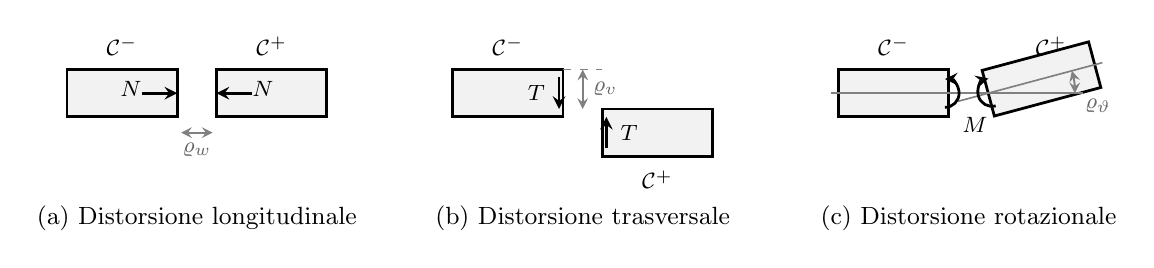
\begin{tikzpicture}[>=stealth, line width=0.8pt, font=\small]
			
			%% ── Parametri geometrici globali ─────────────────────────────────
			\def\Lc{1.40}    % lunghezza del concio (cm)
			\def\Hc{0.60}    % altezza del concio (cm)
			\def\gap{0.50}   % gap tra i due lembi (cm) — distorsione longitudinale
			\def\Wp{4.5}     % larghezza nominale di ciascun pannello (cm)
			\def\Hp{2.5}     % altezza nominale di ciascun pannello (cm)
			\def\GapP{0.4}   % spazio orizzontale tra i pannelli
			
			%% offset per scope
			\def\XPa{0}
			\pgfmathsetmacro{\XPb}{\Wp + \GapP}
			\pgfmathsetmacro{\XPc}{2*(\Wp + \GapP)}
			
			%% =================================================================
			%% PANNELLO (a) — DISTORSIONE LONGITUDINALE varrho_w e forza N
			%% =================================================================
			\begin{scope}[xshift=\XPa cm, yshift=0cm]
				
				%% Coordinate locali del concio
				\pgfmathsetmacro{\xCm}{0.5*\Wp - 0.5*\Lc - 0.5*\gap}
				\pgfmathsetmacro{\xCp}{0.5*\Wp + 0.5*\gap + 0.5*\Lc}
				\pgfmathsetmacro{\xLm}{\xCm - 0.5*\Lc}
				\pgfmathsetmacro{\xRm}{\xCm + 0.5*\Lc}
				\pgfmathsetmacro{\xLp}{\xCp - 0.5*\Lc}
				\pgfmathsetmacro{\xRp}{\xCp + 0.5*\Lc}
				\pgfmathsetmacro{\xMid}{0.5*(\xRm + \xLp)}
				\pgfmathsetmacro{\yQ}{-0.5*\Hc - 0.20}
				
				%% Lembo C^-
				\draw[line width=1.0pt, fill=black!5]
				(\xLm, -0.5*\Hc) rectangle (\xRm, 0.5*\Hc);
				\node[font=\footnotesize, above] at (\xCm, 0.5*\Hc + 0.05) {$\mathcal{C}^{-}$};
				
				%% Lembo C^+
				\draw[line width=1.0pt, fill=black!5]
				(\xLp, -0.5*\Hc) rectangle (\xRp, 0.5*\Hc);
				\node[font=\footnotesize, above] at (\xCp, 0.5*\Hc + 0.05) {$\mathcal{C}^{+}$};
				
				%% Forze N sulle facce interne, sull'asse del concio
				\def\Lf{0.45}
				\pgfmathsetmacro{\xNm}{\xRm - \Lf}
				\pgfmathsetmacro{\xNmlab}{\xRm - 0.5*\Lf}
				\pgfmathsetmacro{\xNp}{\xLp + \Lf}
				\pgfmathsetmacro{\xNplab}{\xLp + 0.5*\Lf}
				
				\draw[->, line width=1.0pt] (\xNm, 0) -- (\xRm, 0);
				\node[font=\footnotesize, left] at (\xNmlab-0.1, 0.05) {$N$};
				
				\draw[->, line width=1.0pt] (\xNp, 0) -- (\xLp, 0);
				\node[font=\footnotesize, right] at (\xNplab+0.1, 0.05) {$N$};
				
				%% Distorsione varrho_w come doppia freccia che apre il gap
				\draw[<->, line width=0.7pt, gray]
				(\xRm + 0.05, \yQ) -- (\xLp - 0.05, \yQ);
				\node[font=\footnotesize, below, color=black!60]
				at (\xMid, \yQ) {$\varrho_w$};
				
				%% Etichetta pannello
				\node[font=\small, below=0.05] at (0.5*\Wp, -1.3)
				{(a) Distorsione longitudinale};
				
			\end{scope}
			
			%% =================================================================
			%% PANNELLO (b) — DISTORSIONE TRASVERSALE varrho_v e taglio T
			%% =================================================================
			\begin{scope}[xshift=\XPb cm, yshift=0cm]
				
				%% Coordinate locali
				\pgfmathsetmacro{\xCm}{0.5*\Wp - 0.5*\Lc - 0.5*\gap}
				\pgfmathsetmacro{\xCp}{0.5*\Wp + 0.5*\gap + 0.5*\Lc}
				\pgfmathsetmacro{\xLm}{\xCm - 0.5*\Lc}
				\pgfmathsetmacro{\xRm}{\xCm + 0.5*\Lc}
				\pgfmathsetmacro{\xLp}{\xCp - 0.5*\Lc}
				\pgfmathsetmacro{\xRp}{\xCp + 0.5*\Lc}
				\pgfmathsetmacro{\xMid}{0.5*(\xRm + \xLp)}
				
				%% Quote verticali: C^- in posizione, C^+ abbassato di gap
				\pgfmathsetmacro{\yCm}{0}
				\pgfmathsetmacro{\yCp}{-\gap}
				\pgfmathsetmacro{\yMtop}{\yCm + 0.5*\Hc}
				\pgfmathsetmacro{\yMbot}{\yCm - 0.5*\Hc}
				\pgfmathsetmacro{\yPtop}{\yCp + 0.5*\Hc}
				\pgfmathsetmacro{\yPbot}{\yCp - 0.5*\Hc}
				\pgfmathsetmacro{\yMidVar}{0.5*(\yMtop + \yPtop)}    % quota etichetta varrho_v
				
				%% Lembo C^- (in posizione)
				\draw[line width=1.0pt, fill=black!5]
				(\xLm, \yMbot) rectangle (\xRm, \yMtop);
				\node[font=\footnotesize, above] at (\xCm, \yMtop + 0.05) {$\mathcal{C}^{-}$};
				
				%% Lembo C^+ (abbassato di gap)
				\draw[line width=1.0pt, fill=black!5]
				(\xLp, \yPbot) rectangle (\xRp, \yPtop);
				\node[font=\footnotesize, below] at (\xCp, \yPbot - 0.05) {$\mathcal{C}^{+}$};
				
				%% Linea tratteggiata di riferimento: prolungamento della cima di C^-
				\draw[dashed, thin, gray]
				(\xRm, \yMtop) -- (\xLp, \yMtop);
				
				%% Doppia freccia verticale per varrho_v: dalla cima di C^- alla cima di C^+
				\draw[<->, line width=0.7pt, gray]
				(\xMid, \yMtop) -- (\xMid, \yPtop);
				%				
				\node[font=\footnotesize, right]
				at (\xMid, \yMidVar) {\textcolor{black!60}{$\varrho_v$}};
				
				%% Frecce T sulle facce interne, verticali
				\def\Lt{0.40}
				%% T su C^- (faccia destra): freccia che parte dall'asse del lembo verso il basso
				\draw[->, line width=1.0pt]
				(\xRm - 0.05, \yCm + 0.5*\Lt) -- (\xRm - 0.05, \yCm - 0.5*\Lt);
				\node[font=\footnotesize, left] at (\xRm - 0.10, \yCm) {$T$};
				
				%% T su C^+ (faccia sinistra): freccia verso l'alto
				\draw[->, line width=1.0pt]
				(\xLp + 0.05, \yCp - 0.5*\Lt) -- (\xLp + 0.05, \yCp + 0.5*\Lt);
				\node[font=\footnotesize, right] at (\xLp + 0.10, \yCp) {$T$};
				
				%% Etichetta pannello
				\node[font=\small, below=0.05] at (0.5*\Wp, -1.3)
				{(b) Distorsione trasversale};
				
			\end{scope}
			
			%% =================================================================
			%% PANNELLO (c) — DISTORSIONE ROTAZIONALE varrho_vartheta e momento M
			%% =================================================================
			\begin{scope}[xshift=\XPc cm, yshift=0cm]
				
				%% Coordinate locali del concio
				\pgfmathsetmacro{\xCm}{0.5*\Wp - 0.5*\Lc - 0.5*\gap}
				\pgfmathsetmacro{\xCp}{0.5*\Wp + 0.5*\gap + 0.5*\Lc}
				\pgfmathsetmacro{\xLm}{\xCm - 0.5*\Lc}
				\pgfmathsetmacro{\xRm}{\xCm + 0.5*\Lc}
				\pgfmathsetmacro{\xLp}{\xCp - 0.5*\Lc}
				\pgfmathsetmacro{\xRp}{\xCp + 0.5*\Lc}
				\pgfmathsetmacro{\xMid}{0.5*(\xRm + \xLp)}
				
				%% Angolo di rotazione di C^+ (in gradi, per visualizzazione)
				\def\angR{15}
				
				%% Lembo C^- (in posizione, orizzontale)
				\draw[line width=1.0pt, fill=black!5]
				(\xLm, -0.5*\Hc) rectangle (\xRm, 0.5*\Hc);
				\node[font=\footnotesize, above] at (\xCm, 0.5*\Hc + 0.05) {$\mathcal{C}^{-}$};
				
				%% Lembo C^+ (ruotato di angR attorno al suo bordo sinistro xLp)
				\begin{scope}[rotate around={\angR:(\xLp,0)}]
					\draw[line width=1.0pt, fill=black!5]
					(\xLp, -0.5*\Hc) rectangle (\xRp, 0.5*\Hc);
				\end{scope}
				%% Etichetta C^+ posizionata fuori dal lembo ruotato
				\node[font=\footnotesize, above]
				at (\xCp + 0.10, 0.5*\Hc + 0.05) {$\mathcal{C}^{+}$};
				
				%% Asse del lembo C^- prolungato a destra (orizzontale)
				\draw[line width=0.6pt, gray]
				(\xLm - 0.10, 0) -- (\xLp + 1.20, 0);
				
				
				
				%% Asse del lembo C^+ prolungato a sinistra (ruotato di angR antioraria)
				\begin{scope}[rotate around={\angR:(\xLp,0)}]
					\draw[line width=0.6pt, gray]
					(\xLp - 0.40, 0) -- (\xRp + 0.10, 0);
				\end{scope}
				
				
				%% Doppia freccia per varrho_vartheta: arco fra i due assi grigi
				\def\rArc{1.10}    % raggio aumentato per spostare l'arco verso destra
				\draw[<->, line width=0.7pt, gray]
				(\xLp + \rArc, 0) arc (0:\angR:\rArc);
				\pgfmathsetmacro{\xLabArc}{\xLp + \rArc + 0.10}
				\pgfmathsetmacro{\yLabArc}{0.5*\rArc*sin(\angR)}
				\node[font=\footnotesize, right] at (\xLabArc-0.1, \yLabArc-0.3) {\textcolor{black!60}{$\varrho_\vartheta$}};
				
				
				
				%% Coppie M sulle facce interne
				\def\rM{0.18}
				\draw[<-, line width=1.0pt]
				([shift={(\xRm - 0.05, 0)}] 90:\rM)
				arc (90:-90:\rM);
				\node[font=\footnotesize, left] at (\xRm +0.8 - \rM, -0.4) {$M$};
				
				%% Su C^+ (faccia sinistra): coppia antioraria  
				\begin{scope}[rotate around={\angR:(\xLp,0)}]
					\draw[<-, line width=1.0pt]
					([shift={(\xLp + 0.05, 0)}] 90:\rM)
					arc (90:270:\rM);
					%\node[font=\footnotesize, right] at (\xLp - 0.40 + \rM, -0.4) {$M$};
				\end{scope}
				
				
				%% Etichetta pannello
				\node[font=\small, below=0.05] at (0.5*\Wp, -1.3)
				{(c) Distorsione rotazionale};
				
			\end{scope}
			
		\end{tikzpicture}%
	}
	\caption{Distorsioni di concio e caratteristiche della 
		sollecitazione duali: la coppia $(\bm{\sigma},\,\bm{\varrho})$ entra 
		nell'identità bilineare con segno discorde.}
	\label{fig:distorsioni_concio}
\end{figure}



\begin{oss}
	Il segno negativo nella~\eqref{eq:lavoro_continuita}
	non è una anomalia ma la conseguenza di due
	convenzioni tradizionali consolidate che non
	è opportuno modificare: quella delle
	caratteristiche della sollecitazione --- ereditate
	dalla meccanica dei solidi deformabili e riferite
	all'elemento di trave --- e quella delle
	distorsioni --- riferite alla discontinuità
	cinematica come differenza $\mathcal{C}^+ -
	\mathcal{C}^-$. Nei capitoli sul TLV applicato
	alla trave deformabile questo segno sarà
	tenuto in conto esplicitamente.
\end{oss}

\begin{oss}
	La struttura duale --- tre condizioni cinematiche,
	tre reazioni incognite --- è la stessa del
	vincolo di rigidità introdotto nel
	\CAPref{cap:vincoli_CR} e dell'incastro interno
	del catalogo dei vincoli. La differenza è di
	natura fisica: il vincolo di rigidità è una
	proprietà diffusa sulla sezione, mentre l'incastro
	interno è un dispositivo concentrato. In entrambi
	i casi la struttura duale è la stessa.
\end{oss}


%----------------------------------------------------------------------------------------------------------------------------
\subsection{Il metodo per equivalenza}
\label{sec:caratteristiche_calcolo}
%----------------------------------------------------------------------------------------------------------------------------

Le reazioni del vincolo di rigidità in una singola
sezione $S$ --- forza normale $N(S)$, taglio $T(S)$
e momento flettente $M(S)$ --- descrivono lo stato
di sollecitazione interna \emph{in quel punto}.
Nella pratica strutturale interessa però conoscere
la distribuzione completa $N(z)$, $T(z)$, $M(z)$
lungo tutta la linea d'asse: è questa distribuzione
che consente di individuare le sezioni critiche,
valutare la resistenza della trave e interpretare
il comportamento strutturale globale. Il calcolo
deve quindi essere ripetuto per ogni sezione $z$,
e il risultato è una funzione --- il
\emph{diagramma} della caratteristica --- non un
valore isolato. Il \emph{metodo per equivalenza}\index{metodo!per equivalenza|textbf}
fornisce lo strumento sistematico per costruire
questi diagrammi.


Sia la trave globalmente in equilibrio sotto l'azione
di un sistema di forze esterne --- attive e reattive.
Indichiamo con $Z^\pm$, $Y^\pm$ e $\mu^\pm$ le
componenti della risultante e del momento risultante
di tutte le forze esterne agenti rispettivamente sui
tratti $\mathcal{C}^+$ e $\mathcal{C}^-$, calcolate
nel riferimento intrinseco rispetto al punto $S$:
\begin{equation}\label{eq:equilibrio_globale}
	Z^+ + Z^- = 0, \qquad
	Y^+ + Y^- = 0, \qquad
	\mu^+ + \mu^- = 0.
\end{equation}
Le~\eqref{eq:equilibrio_globale} esprimono
l'equilibrio globale della trave: la risultante e
il momento risultante di tutte le forze esterne
sono nulli.

Pratichiamo ora idealmente il taglio in $S$:
i due tratti $\mathcal{C}^-$ e $\mathcal{C}^+$
diventano due corpi distinti. L'equilibrio di
$\mathcal{C}^-$ richiede che $\mathcal{C}^+$
gli trasmetta attraverso la sezione $S$ una forza
risultante e un momento risultante tali da
bilanciare $Z^-$, $Y^-$ e $\mu^-$. Dalle
\eqref{eq:equilibrio_globale}:
\begin{equation}\label{eq:NTM_def}
	\boxed{N \coloneqq Z^+ = -Z^-, \qquad
		T \coloneqq Y^+ = -Y^-, \qquad
		M \coloneqq \mu^+ = -\mu^-.}
\end{equation}

Le~\eqref{eq:NTM_def} rivelano la \emph{doppia
	natura} delle caratteristiche della sollecitazione:
\begin{itemize}[nosep]
	\item \textbf{Lettura interna}: $N$, $T$, $M$
	sono le reazioni del vincolo di rigidità
	trasmesse da $\mathcal{C}^+$ a $\mathcal{C}^-$
	attraverso la sezione $S$ --- la ``colla'' che
	tiene uniti i due tratti;
	\item \textbf{Lettura esterna}: $N$, $T$, $M$
	sono le componenti della risultante e del
	momento risultante di tutte le forze esterne
	agenti su $\mathcal{C}^+$ --- la ``somma'' di
	tutto ciò che agisce a destra della sezione.
	Equivalentemente, $-N$, $-T$, $-M$ sono
	le stesse grandezze riferite a $\mathcal{C}^-$.
\end{itemize}

La convenzione di segno adottata è illustrata
nella \FIGref{fig:concio_NTM}: sulla faccia
destra del concio --- normale uscente $+z^e$ ---
$N$, $T$, $M$ agiscono nei versi positivi convenuti;
sulla faccia sinistra --- normale uscente $-z^e$
--- i versi sono opposti. Il calcolo per
equivalenza si esegue sommando algebricamente
le forze esterne su uno dei due tratti, scegliendo
quello più conveniente.

\begin{figure}[htbp]
	\centering
	\begin{tikzpicture}[>=Stealth, line width=0.8pt, scale=0.80]
		
		% ── Trave AB in alto ─────────────────────────────
		\draw[thick] (0, 3.5) -- (8, 3.5);
		\draw[dashed, thick] (0, 3.35) -- (8, 3.35);
		\fill (0, 3.5) circle (2pt) node[above=4pt] {$A$};
		\fill (8, 3.5) circle (2pt) node[above=4pt] {$B$};
		
		% Linea tratteggiata che collega trave al concio
		\draw[dashed, gray!50, thin] (3.7, 3.35) -- (3.7, 2.5);
		\draw[dashed, gray!50, thin] (4.3, 3.35) -- (4.3, 2.5);
		
		% ── Concio assottigliato ─────────────────────────
		\draw[thick] (3.7, 0.5) rectangle (4.3, 2.5);
		
		% Tratteggio fibra inferiore concio
		\draw[dashed, thick] (3.7, 0.35) -- (4.3, 0.35);
		
		% ── Faccia destra (normale +z^e) ─────────────────
		% N: verso destra
		\draw[->, line width=1.6pt]
		(4.3, 1.5) -- (5.5, 1.5);
		\node[above=2pt] at (5.0, 1.5) {$N$};
		
		% T: verso il basso
		\draw[->, line width=1.6pt]
		(4.3, 1.5) -- (4.3, 0.3);
		\node[right=2pt] at (4.3, 0.9) {$T$};
		
		% M: quarto di cerchio da T a N
		\draw[->, line width=1.6pt]
		(4.3, 0.3) arc[start angle=270,
		end angle=360, radius=1.2];
		\node[right=2pt] at (5.25, 0.85) {$M$};
		
		% ── Faccia sinistra (normale -z^e) ────────────────
		% N: verso sinistra
		\draw[->, line width=1.6pt]	(3.7, 1.5) -- (2.5, 1.5);	\node[below=2pt] at (3.0, 1.5) {$N$};
		
		% T: verso l'alto
		\draw[->, line width=1.6pt]
		(3.7, 1.5) -- (3.7, 2.7);
		\node[left=2pt] at (3.7, 2.1) {$T$};
		
		% M: quarto di cerchio da N a T
		\draw[->, line width=1.6pt]
		(2.5, 1.5) arc[start angle=180,
		end angle=90, radius=1.2];
		\node[left=2pt] at (2.85, 2.45) {$M$};
		
	\end{tikzpicture}
	\caption{Concio di trave e convenzione di segno
		delle caratteristiche della sollecitazione.
		Sulla faccia destra (normale uscente $+z^e$)
		$N$, $T$, $M$ sono positivi se concordi con
		gli assi del riferimento intrinseco; sulla
		faccia sinistra (normale uscente $-z^e$)
		i versi positivi sono opposti.}
	\label{fig:concio_NTM}
\end{figure}


\begin{oss}
	Le caratteristiche della sollecitazione $N$, $T$, $M$
	sono definite sulla faccia destra del concio ---
	quella con normale uscente $+z^e$ --- e sono positive
	nei versi indicati nella \FIGref{fig:concio_NTM}:
	$N$ di trazione, $T$ diretto nel verso $+y^e$, $M$
	nel verso che tende ad allungare le fibre inferiori.
	Le distorsioni $\varrho_w$, $\varrho_v$,
	$\varrho_\vartheta$ sono invece definite come
	differenze $\mathcal{C}^+ - \mathcal{C}^-$: sono
	positive nel verso in cui il tratto destro si
	discosta dal tratto sinistro.
	Le due convenzioni hanno orientamenti opposti:
	un $N > 0$ (trazione) tende a resistere a un
	allungamento relativo $\varrho_w > 0$, e il loro
	prodotto contribuisce negativamente al lavoro
	virtuale --- è questo il contenuto del segno
	negativo nella~\eqref{eq:lavoro_continuita}.
	I versi positivi di $N$, $T$, $M$ sono scelti in
	accordo con la convenzione della meccanica dei
	solidi deformabili, la cui motivazione fisica ---
	legata agli effetti deformativi sul concio
	infinitesimo --- è sviluppata nel Volume~II.
\end{oss}


\begin{oss}
	Il calcolo di $N$, $T$, $M$ per equivalenza
	si fonda sull'equilibrio globale della trave:
	le condizioni~\eqref{eq:eq_glob_z}--\eqref{eq:eq_glob_mu}
	rendono possibile il calcolo delle reazioni
	vincolari e, a partire da esse, la determinazione
	delle caratteristiche della sollecitazione
	in ogni sezione.
\end{oss}

\begin{oss}
	Le due letture sono equivalenti per l'equilibrio
	--- è esattamente il contenuto
	delle~\eqref{eq:NTM_def} --- ma hanno ruoli
	diversi nella pratica del calcolo. La lettura
	interna descrive la fisica della trasmissione
	delle forze attraverso la sezione; la lettura
	esterna fornisce il metodo operativo per
	calcolare $N$, $T$, $M$ in ogni sezione:
	è sufficiente sommare le forze esterne su uno
	dei due tratti, scegliendo quello più conveniente.
	Nei sistemi isostatici, dove le reazioni sono
	note, il calcolo si riduce a una somma algebrica.
\end{oss}

\begin{oss}
	L'equivalenza fra le due espressioni in
	ciascuna delle~\eqref{eq:NTM_def} --- 
	$Z^+ = -Z^-$, $Y^+ = -Y^-$, $\mu^+ = -\mu^-$
	--- è anche una \emph{verifica}: calcolando
	$N$, $T$, $M$ da sinistra e da destra si deve
	ottenere lo stesso risultato. Una discrepanza
	segnala un errore nel calcolo delle reazioni
	o nell'applicazione delle forze esterne.
\end{oss}


\paragraph{Condizioni al contorno.}
Le equazioni~\eqref{eq:NTM_def} si specializzano
agli estremi della trave fornendo le
\emph{condizioni al contorno}\index{condizioni al contorno} per le caratteristiche
della sollecitazione. Siano $Z_A$, $Y_A$, $\mu(A)$
le componenti della risultante e del momento
risultante delle forze esterne applicate
all'estremo sinistro $A$, e $Z_B$, $Y_B$, $\mu(B)$
quelle all'estremo destro $B$:
\begin{itemize}[nosep]
	\item all'estremo destro $B$ la sezione ha
	normale uscente $+z^e$: le caratteristiche
	della sollecitazione sono \emph{concordi} con
	le forze esterne:
	\begin{equation}\label{eq:cc_destra}
		N(B) = Z_B, \qquad
		T(B) = Y_B, \qquad
		M(B) = \mu(B);
	\end{equation}
	\item all'estremo sinistro $A$ la sezione ha
	normale uscente $-z^e$: le caratteristiche
	della sollecitazione sono \emph{discordi} con
	le forze esterne:
	\begin{equation}\label{eq:cc_sinistra}
		N(A) = -Z_A, \qquad
		T(A) = -Y_A, \qquad
		M(A) = -\mu(A).
	\end{equation}
\end{itemize}

\begin{oss}
	Le condizioni al contorno~\eqref{eq:cc_destra}
	e~\eqref{eq:cc_sinistra} sono il punto di
	partenza del calcolo per equivalenza: una volta
	note le reazioni vincolari agli estremi, i valori
	di $N$, $T$, $M$ agli estremi sono immediatamente
	determinati, e da questi si procede verso
	l'interno della trave sommando le forze esterne
	sul tratto considerato.
\end{oss}






%----------------------------------------------------------------------------------------------------------------------------
\subsection{Salto ai punti di singolarità}
\label{sec:salto_singolarita}
%----------------------------------------------------------------------------------------------------------------------------

In una sezione $S$ in cui agiscono una forza
concentrata di componenti $Z(S)$ nella direzione
$z^e$ e $Y(S)$ nella direzione $y^e$, e una coppia
concentrata $\mu(S)$, le caratteristiche della
sollecitazione presentano una \emph{discontinuità}\index{salto!delle caratteristiche della sollecitazione}.
Per determinarne l'entità si considera l'equilibrio
di un concio di lunghezza $2\varepsilon$ centrato
in $S$, compreso tra le sezioni $S^-$ (a sinistra)
e $S^+$ (a destra), e si compie il limite
$\varepsilon \to 0$.

Nel limite, i contributi dei carichi distribuiti
$q$, $p$, $c$ scompaiono perché proporzionali a
$2\varepsilon \to 0$; rimangono solo i termini
concentrati in $S$. L'equilibrio nella direzione
$z^e$, nella direzione $y^e$ e dei momenti rispetto
a $S$ fornisce:
\begin{equation}
	\boxed{\begin{aligned}
			\llbracket N \rrbracket_S &\coloneqq
			N(S^+) - N(S^-) = -Z(S),\\
			\llbracket T \rrbracket_S &\coloneqq
			T(S^+) - T(S^-) = -Y(S),\\
			\llbracket M \rrbracket_S &\coloneqq
			M(S^+) - M(S^-) = -\mu(S),
	\end{aligned}}
	\label{eq:salto_NTM}
\end{equation}

\begin{oss}
	Le~\eqref{eq:salto_NTM}
	sono equazioni di \emph{equilibrio locale
		algebrico} nel punto di singolarità $S$:
	esprimono il bilancio delle forze e dei momenti
	in un intorno infinitesimo di $S$. Il segno
	negativo è conseguenza della convenzione di
	segno adottata per le caratteristiche della
	sollecitazione: $N$, $T$, $M$ sono positivi
	sulla faccia con normale uscente $+z^e$, mentre
	$Z(S)$, $Y(S)$, $\mu(S)$ sono positivi nei
	versi degli assi del riferimento intrinseco.
	Una forza $Y(S) > 0$ --- verso il basso ---
	produce un salto negativo del taglio:
	$\llbracket T \rrbracket_S = -Y(S) < 0$.
\end{oss}


\begin{figure}[htbp]
	\centering
	\begin{tikzpicture}[>=Stealth, line width=0.8pt,
		scale=1.1]
		
		% ── Trave AB con carichi distribuiti ─────────────
		\draw[thick] (0,0) -- (9,0);
		\draw[dashed, thick] (0,-0.18) -- (9,-0.18);
		\fill (0,0) circle (2pt);
		\node[below=6pt] at (0,0) {$A$};
		\fill (9,0) circle (2pt);
		\node[below=6pt] at (9,0) {$B$};
		
		% p(z)
		\draw[thick, domain=0:9, samples=100]
		plot (\x, {1.2 + 0.5*sin(\x*40)});
		\foreach \x in {0.3, 0.9, 1.5, 2.1, 2.7, 3.3,
			3.9, 4.5, 5.1, 5.7, 6.3, 6.9,
			7.5, 8.1, 8.7}{
			\pgfmathsetmacro{\h}{1.2 + 0.5*sin(\x*40)}
			\draw[->, thin] (\x, \h) -- (\x, 0);
		}
		\node[right] at (9.1, {1.2+0.5*sin(360)}) {$p(z)$};
		
		% q(z)
		\foreach \x in {0.3, 0.9, 1.5, 2.1, 2.7, 3.3,
			3.9, 4.5, 5.1, 5.7, 6.3, 6.9,
			7.5, 8.1, 8.7}{
			\draw[->, thin] (\x-0.35, 0.35) -- (\x, 0.35);
		}
		\draw[thick] (0,0.35) -- (9,0.35);
		\node[right] at (9.1, 0.35) {$q(z)$};
		
		% c(z)
		\foreach \x in {0.5, 1.3, 2.1, 2.9, 3.7,
			5.3, 6.1, 6.9, 7.7, 8.5}{
			\draw[->] (\x+0.18, 0.72)
			arc[start angle=0, end angle=180,
			radius=0.18];
		}
		\node[right] at (9.1, 0.72) {$c(z)$};
		
		% ── Forze concentrate in S ────────────────────────
		% S sulla trave
		\fill (4.5, 0) circle (2pt);
		\node[above=4pt] at (4.5, 0) {$S$};
		
		% Z(S): verso destra
		\draw[->, line width=1.4pt]
		(4.5, 0.0) -- (5.5, 0.0);
		\node[below=2pt, font=\small] at (5.0, 0.0) {$Z(S)$};
		
		% Y(S): verso il basso
		\draw[->, line width=1.4pt]
		(4.5, 0) -- (4.5, -0.9);
		\node[right=2pt, font=\small] at (3.5,-0.45) {$Y(S)$};
		
		% mu(S): coppia antioraria
		\draw[->] (4.88, 0.55)
		arc[start angle=0, end angle=180,
		radius=0.38];
		\node[above=2pt, font=\small] at (4.5, 0.7) {$\mu(S)$};
		
		% Linee tratteggiate verso concio
		\draw[dashed, gray!50, thin] (3.3,-0.18) -- (2.0,-2.0);
		\draw[dashed, gray!50, thin] (5.7,-0.18) -- (7.0,-2.0);
		
		% ── Concio di larghezza 2epsilon ──────────────────
		\draw[thick] (2.0,-3.8) rectangle (7.0,-2.0);
		\draw[dashed, thick] (2.0,-4.0) -- (7.0,-4.0);
		
		% Centro del concio = S
		\coordinate (S) at (4.5,-2.9);
		
		% Etichette S^- e S^+
		\node[below=4pt, font=\small] at (2.2,-2.6) {$S^-$};
		\node[below=4pt, font=\small] at (6.8,-2.6) {$S^+$};
		
		% Quote epsilon
		\draw[thin] (4.5,-3.8) -- (4.5,-4.3);
		\draw[|<->|, thin] (2.0,-4.2) -- (4.5,-4.2)
		node[midway, below=2pt] {$\varepsilon$};
		\draw[|<->|, thin] (4.5,-4.2) -- (7.0,-4.2)
		node[midway, below=2pt] {$\varepsilon$};
		
		% ── Forze concentrate al centro ───────────────────
		% Z(S)
		\draw[->, line width=1.4pt]
		(S) -- ++(1.2, 0);
		\node[above=2pt, font=\small] at (5.5,-2.9) {$Z(S)$};
		
		% Y(S)
		\draw[->, line width=1.4pt]
		(S) -- ++(0, -0.8);
		\node[right=2pt, font=\small] at (4.5,-3.3) {$Y(S)$};
		
		% mu(S)
		\draw[->] (4.88,-2.45)
		arc[start angle=0, end angle=180,
		radius=0.38];
		\node[above=2pt, font=\small] at (4.5,-2.8) {$\mu(S)$};
		
		% ── Faccia sinistra S^- ───────────────────────────
		% N
		\draw[->, line width=1.6pt]
		(2.0,-2.9) -- (0.7,-2.9);
		\node[above=2pt, font=\small] at (1.2,-3.6) {$N(S^-)$};
		
		% T
		\draw[->, line width=1.6pt]
		(2.0,-2.9) -- (2.0,-1.7);
		\node[left=2pt, font=\small] at (2.2,-2.3) {$T(S^-)$};
		
		% M
		\draw[->, line width=1.6pt]
		(0.7,-2.9) arc[start angle=180,
		end angle=90, radius=1.2];
		\node[left=2pt, font=\small] at (1.15,-1.9) {$M(S^-)$};
		
		% ── Faccia destra S^+ ─────────────────────────────
		% N
		\draw[->, line width=1.6pt]
		(7.0,-2.9) -- (8.3,-2.9);
		\node[above=2pt, font=\small] at (7.8,-2.9) {$N(S^+)$};
		
		% T
		\draw[->, line width=1.6pt]
		(7.0,-2.9) -- (7.0,-4.1);
		\node[right=2pt, font=\small] at (6.85,-3.4) {$T(S^+)$};
		
		% M
		\draw[->, line width=1.6pt]
		(7.0,-4.1) arc[start angle=270,
		end angle=360, radius=1.2];
		\node[right=2pt, font=\small] at (7.9,-3.6) {$M(S^+)$};
		
	\end{tikzpicture}
	\caption{Trave con carichi distribuiti e forze
		concentrate $Z(S)$, $Y(S)$, $\mu(S)$ in $S$
		(in alto). Concio di lunghezza $2\varepsilon$
		centrato in $S$ (ingrandimento in basso):
		nel limite $\varepsilon \to 0$ i carichi
		distribuiti scompaiono e rimangono solo le
		forze concentrate. L'equilibrio fornisce le
		equazioni di salto
		\eqref{eq:salto_NTM}.}
	\label{fig:concio_salto}
\end{figure}



%----------------------------------------------------------------------------------------------------------------------------
\subsection{Equazioni indefinite di equilibrio}
\label{sec:eq_indefinite}
%----------------------------------------------------------------------------------------------------------------------------

Si dice \emph{tratto regolare}\index{tratto regolare|textbf} un tratto della trave
in cui:
\begin{itemize}[nosep]
	\item le caratteristiche della sollecitazione
	$N$, $T$, $M$ sono funzioni continue di $z$
	--- non vi sono discontinuità statiche, ovvero
	forze o coppie concentrate;
	\item le densità di carico $q(z)$, $p(z)$,
	$c(z)$ sono funzioni continue di $z$ --- non
	vi sono discontinuità nelle leggi di carico.
\end{itemize}

In un tratto regolare è possibile scrivere le
equazioni di equilibrio in forma differenziale.
Si considera l'equilibrio di un elemento
infinitesimo di trave di lunghezza $\dd z$,
compreso tra le sezioni $P$ (di ascissa $z$) e
$Q$ (di ascissa $z + \dd z$), come illustrato
nella \FIGref{fig:concio_eq_indefinite}.


\begin{figure}[htbp]
	\centering
	\begin{tikzpicture}[>=Stealth, line width=0.8pt,
		scale=1.1]
		
		% ── Trave AB con carichi distribuiti ─────────────
		\draw[thick] (0,0) -- (9,0);
		\draw[dashed, thick] (0,-0.18) -- (9,-0.18);
		\fill (0,0) circle (2pt);
		\node[below=6pt] at (0,0) {$A$};
		\fill (9,0) circle (2pt);
		\node[below=6pt] at (9,0) {$B$};
		
		% p(z)
		\draw[thick, domain=0:9, samples=100]
		plot (\x, {1.2 + 0.5*sin(\x*40)});
		\foreach \x in {0.3, 0.9, 1.5, 2.1, 2.7, 3.3,
			3.9, 4.5, 5.1, 5.7, 6.3, 6.9,
			7.5, 8.1, 8.7}{
			\pgfmathsetmacro{\h}{1.2 + 0.5*sin(\x*40)}
			\draw[->, thin] (\x, \h) -- (\x, 0);
		}
		\node[right] at (9.1, {1.2+0.5*sin(360)}) {$p(z)$};
		
		% q(z)
		\foreach \x in {0.3, 0.9, 1.5, 2.1, 2.7, 3.3,
			3.9, 4.5, 5.1, 5.7, 6.3, 6.9,
			7.5, 8.1, 8.7}{
			\draw[->, thin] (\x-0.35, 0.35) -- (\x, 0.35);
		}
		\draw[thick] (0,0.35) -- (9,0.35);
		\node[right] at (9.1, 0.35) {$q(z)$};
		
		% c(z) — archi antiorari
		\foreach \x in {0.5, 1.3, 2.1, 2.9, 3.7, 4.5,
			5.3, 6.1, 6.9, 7.7, 8.5}{
			\draw[->] (\x+0.18, 0.72)
			arc[start angle=0, end angle=180,
			radius=0.18];
		}
		\node[right] at (9.1, 0.72) {$c(z)$};
		
		% Punti P e Q
		\draw[thin] (4.0, -0.3) -- (4.0, 0.1);
		\draw[thin] (5.2, -0.3) -- (5.2, 0.1);
		%\node[below=2pt] at (3.8, -0.3) {$P$};
		\node[below=2pt] at (4.0, -0.12) {\footnotesize$(z)$};
		%\node[below=2pt] at (5.4, -0.3) {$Q$};
		\node[below=2pt] at (5.3, -0.12)
		{\footnotesize$(z{+}\dd z)$};
		\draw[|<->|, thin] (4.0,-0.75) -- (5.2,-0.75)
		node[midway, below=2pt] {$\dd z$};
		
		% Linee tratteggiate verso concio
		\draw[dashed, gray!50, thin] (4.0,-0.18) -- (2.0,-2.0);
		\draw[dashed, gray!50, thin] (5.2,-0.18) -- (7.0,-2.0);
		
		% ── Concio ingrandito (più corto) ─────────────────
		\draw[thick] (2.0,-3.8) rectangle (7.0,-2.0);
		\draw[dashed, thick] (2.0,-4.0) -- (7.0,-4.0);
		
		% Centro del concio
		\coordinate (C) at (4.5,-2.9);
		
		% Etichette P e Q sulle facce
		\node[below=4pt] at (2.2,-2.6) {$P$};
		\node[below=4pt] at (6.8,-2.6) {$Q$};
		
		% c dz: coppia antioraria sopra il centro
		\draw[->] (4.85,-2.8)
		arc[start angle=0, end angle=180,
		radius=0.38];
		\node[above=2pt, font=\small] at (4.5,-2.6) {$c(z)\,\dd z$};
		
		% q dz: freccia da centro verso destra
		\draw[->, line width=1.2pt]
		(C) -- ++(1.5, 0)
		node[above=2pt, font=\small] {$q(z)\,\dd z$};
		
		%p dz: freccia dal centro verso il basso
		\draw[->, line width=1.2pt]
		(C) -- ++(0, -0.9)
		node[pos=0.5, right=2pt, font=\small] {$p(z)\,\dd z$};
		
		% ── Faccia sinistra P ─────────────────────────────
		% N
		\draw[->, line width=1.6pt]
		(2.0,-2.9) -- (0.7,-2.9);
		\node[above=2pt, font=\small] at (1.2,-2.9) {$N$};
		
		% T
		\draw[->, line width=1.6pt]
		(2.0,-2.9) -- (2.0,-1.7);
		\node[left=2pt, font=\small] at (2.0,-2.3) {$T$};
		
		% M
		\draw[->, line width=1.6pt]
		(0.7,-2.9) arc[start angle=180,
		end angle=90, radius=1.2];
		\node[left=2pt, font=\small] at (0.95,-1.9) {$M$};
		
		% ── Faccia destra Q ───────────────────────────────
		% N+dN
		\draw[->, line width=1.6pt]
		(7.0,-2.9) -- (8.3,-2.9);
		\node[above=2pt, font=\small] at (7.8,-2.9) {$N{+}\dd N$};
		
		% T+dT
		\draw[->, line width=1.6pt]
		(7.0,-2.9) -- (7.0,-4.1);
		\node[right=2pt, font=\small] at (6.85,-3.4) {$T{+}\dd T$};
		
		% M+dM
		\draw[->, line width=1.6pt]
		(7.0,-4.1) arc[start angle=270,
		end angle=360, radius=1.2];
		\node[right=2pt, font=\small] at (7.9,-3.6) {$M{+}\dd M$};
		
	\end{tikzpicture}
	\caption{Trave con carichi distribuiti $p(z)$,
		$q(z)$, $c(z)$ (in alto) e concio infinitesimo
		di lunghezza $\dd z$ tra le sezioni $P$ e $Q$
		(ingrandimento in basso). Le risultanti dei
		carichi distribuiti $p(z)\,\dd z$, $q(z)\,\dd z$,
		$c(z)\,\dd z$ sono applicate al centro del
		concio. Sulla faccia $P$ le caratteristiche
		della sollecitazione agiscono con verso negativo;
		sulla faccia $Q$ con verso positivo incrementate
		di $\dd N$, $\dd T$, $\dd M$.}
	\label{fig:concio_eq_indefinite}
\end{figure}


Le forze agenti sull'elemento sono:
\begin{itemize}[nosep]
	\item sulla faccia sinistra: $-N(z)$, $-T(z)$,
	$-M(z)$;
	\item sulla faccia destra: $N(z+\dd z)$,
	$T(z+\dd z)$, $M(z+\dd z)$;
	\item sul volume dell'elemento: $q\,\dd z$
	nella direzione $z^e$, $p\,\dd z$ nella
	direzione $y^e$, $c\,\dd z$ come coppia.
\end{itemize}

L'equilibrio della risultante in $z^e$, in $y^e$
e dei momenti rispetto alla sezione destra dà,
al primo ordine in $\dd z$\index{equazioni indefinite di equilibrio|textbf}:
\begin{equation}\label{eq:eq_indefinite}
	\boxed{\frac{\dd N}{\dd z} + q = 0,
		\qquad
		\frac{\dd T}{\dd z} + p = 0,
		\qquad
		\frac{\dd M}{\dd z} - T + c = 0.}
\end{equation}

\begin{oss}
	Le~\eqref{eq:eq_indefinite} sono equazioni di
	\emph{statica} scritte nella configurazione
	di riferimento: non presuppongono alcuna
	ipotesi di deformabilità e sono valide per
	qualsiasi trave --- rigida o deformabile ---
	nell'ipotesi di piccoli spostamenti.
\end{oss}

\begin{oss}
	Le equazioni di salto~\eqref{eq:salto_NTM}
	e le equazioni indefinite~\eqref{eq:eq_indefinite}
	sono entrambe equazioni di \emph{equilibrio
		locale}: le prime sono equazioni algebriche
	valide nei punti di singolarità; le seconde
	sono equazioni differenziali valide nei tratti
	regolari. Insieme descrivono completamente
	l'equilibrio locale della trave in ogni punto.
\end{oss}


Le equazioni indefinite~\eqref{eq:eq_indefinite}
non vengono integrate in questo volume: il calcolo
di $N$, $T$, $M$ in ogni sezione si esegue per
\emph{equivalenza} --- sommando le forze esterne
su uno dei due tratti come nelle~\eqref{eq:NTM_def}
--- che è sufficiente per la trave rigida e più
diretto dell'integrazione. L'approccio analitico
per integrazione --- che diventa necessario quando
si introduce la legge costitutiva della trave
deformabile --- è sviluppato nel Volume~II.
Le equazioni indefinite sono tuttavia utili
per ricavare informazioni qualitative sulla
struttura dei diagrammi di $N$, $T$, $M$
senza calcolarli esplicitamente:
\begin{itemize}[nosep]
	\item dove $q = 0$: $N$ è uniforme;
	\item dove $p = 0$: $T$ è uniforme,
	$M$ è lineare;
	\item dove $p$ è uniforme: $T$ è lineare,
	$M$ è parabolico;
	\item dove $p$ è lineare: $T$ è parabolico,
	$M$ è cubico;
	\item dove $T = 0$ (e $c = 0$): $M$ ha un
	punto di stazionarietà --- massimo o minimo
	--- che individua la sezione maggiormente
	sollecitata a momento flettente;
	\item dove $c = 0$: la curvatura del diagramma
	di $M$ è $\frac{\dd^2 M}{\dd z^2} = -p$;
	poiché il semiasse positivo di $M$ è tracciato
	verso le fibre inferiori, il diagramma ha
	\emph{concavità verso l'alto} dove $p > 0$
	(carico verso la fibra inferiore) e
	\emph{concavità verso il basso} dove $p < 0$.
\end{itemize}




\begin{esempio}[Trave isostatica con distorsione e carichi esterni] \label{sec:esempio_completo}
	Una trave rettilinea $AB$ di lunghezza $\ell$ è vincolata
	con una cerniera in $A$ e un carrello verticale in $B$.
	In una sezione interna $S$, posta a distanza $\ell/3$
	dall'estremo $A$, è imposta una distorsione rotazionale
	$\varrho_\vartheta > 0$. Agiscono inoltre un carico
	distribuito uniforme $\bar p$ nella direzione $+y^e$
	(verso la fibra inferiore) su tutta la lunghezza e una
	forza concentrata $F = 2\bar p\ell$ nella direzione
	$+y^e$ applicata in $S$
	(\FIGref{fig:esempio_completo}\,(a)).
	Si determinino la configurazione deformata e i diagrammi
	delle caratteristiche della sollecitazione $T(z)$ e $M(z)$.
	
	\begin{svolgimento}
		
		\esottotit{Problema cinematico.}
		Il problema cinematico riguarda la configurazione deformata
		dei due tratti in seguito alla distorsione $\varrho_\vartheta$.
		I carichi esterni non entrano nella cinematica del corpo rigido:
		a parità di vincoli e distorsioni, la configurazione è
		indipendente dai carichi applicati.
		
		I vincoli esterni, espressi nel riferimento intrinseco
		$(y^e,\, z^e)$, impongono $v(A) = w(A) = v(B) = 0$.
		I due tratti ruotano rigidamente; scegliendo il polo in $A$,
		lo spostamento verticale vale
		\begin{equation*}
			v(z) = -\vartheta^- z
			\qquad \Bigl(0 \le z \le \tfrac{\ell}{3}\Bigr),
		\end{equation*}
		\begin{equation*}
			v(z) = -\vartheta^-\tfrac{\ell}{3}
			- \vartheta^+\Bigl(z - \tfrac{\ell}{3}\Bigr)
			\qquad \Bigl(\tfrac{\ell}{3} \le z \le \ell\Bigr),
		\end{equation*}
		dove $\vartheta^+ = \vartheta^- + \varrho_\vartheta$.
		La condizione $v(\ell) = 0$ fornisce
		$\vartheta^- = -\tfrac{2}{3}\varrho_\vartheta$ e
		$\vartheta^+ = \tfrac{1}{3}\varrho_\vartheta$:
		i due tratti ruotano in versi opposti, e lo spostamento
		massimo si raggiunge in $S$ con valore
		$v(S) = \tfrac{2}{9}\varrho_\vartheta\ell$.
		La configurazione deformata è mostrata in
		\FIGref{fig:esempio_completo}\,(b).
		
		\esottotit{Problema statico.}
		Il problema statico riguarda le caratteristiche della
		sollecitazione prodotte dai carichi esterni $\bar p$ e $F$.
		Per un sistema isostatico le distorsioni non contribuiscono
		alle caratteristiche: il problema statico è indipendente
		da $\varrho_\vartheta$
		(Oss.~\ref{oss:distorsione_isostatica}).
		
		\esottotit{Calcolo delle reazioni.}
		In assenza di forza assiale, $Z_A = 0$. Le equazioni di
		equilibrio globale~\eqref{eq:eq_glob_y}--\eqref{eq:eq_glob_mu},
		con $Y_A$ e $Y_B$ positivi verso l'alto, danno
		\begin{equation*}
			Y_A = \tfrac{11}{6}\bar p\ell, \qquad
			Y_B = \tfrac{7}{6}\bar p\ell.
		\end{equation*}
		
		\begin{figure}[!htbp]
			\centering
			\resizebox{\textwidth}{!}{%
				\begin{tikzpicture}[
					>=stealth, line width=0.8pt,
					trave/.style={line width=1.5pt, line cap=round,
						line join=round, black},
					travedef/.style={line width=1.5pt, line cap=round,
						line join=round, gray!55},
					terra/.style={line width=0.8pt, black},
					carico/.style={->, >=stealth, line width=1.2pt, black},
					quota/.style={<->, >=stealth, thin, gray!60},
					nodoV/.style={circle, fill=white, draw=black,
						inner sep=0pt, minimum size=4pt,
						line width=0.7pt}, diag/.style={line width=0.7pt, black},
					hatch/.style={line width=0.3pt, gray!50},
					segno/.style={circle, draw=black, inner sep=0.8pt,
						line width=0.5pt, font=\scriptsize},
					etichetta/.style={circle, draw=black, inner sep=2.5pt,
						line width=0.8pt, font=\small}
					]
					
					%% ===============================================================
					%% PANNELLO (a) — Schema: geometria, vincoli, carichi, distorsione
					%% ===============================================================
					\begin{scope}[xshift=0cm, yshift=0cm]
						
						\def\L{6.0}
						\pgfmathsetmacro{\xS}{\L/3}
						
						%% linea d'asse + fibra inferiore
						\draw[trave] (0,0) -- (\L,0);
						\draw[dashed, thin] (0,-0.1) -- (\L,-0.1);
						
						%% ferri di chiamata grigi (verso la quota)
						\draw[very thin, gray!50] (0  ,-0.05) -- (0  ,-1.02);
						\draw[very thin, gray!50] (\xS,-0.05) -- (\xS,-1.02);
						\draw[very thin, gray!50] (\L ,-0.05) -- (\L ,-1.02);
						
						%% cerniera esterna in A
						\draw[terra] (0,0) -- ++(-0.22,-0.38) -- ++(0.44,0) -- cycle;
						\draw[terra] (-0.30,-0.38) -- (0.30,-0.38);
						\foreach \x in {-0.24,-0.12,0,0.12,0.24}
						\draw[very thin, black] (\x,-0.38) -- ++(-0.09,-0.11);
						\node[nodoV] at (0,0) {};
						\node[above left=1pt and 2pt, font=\small] at (0,0) {$A$};
						
						%% carrello verticale in B (canone ridotto)
						\draw[terra] (\L,0) -- ++(-0.25,-0.36) -- ++(0.50,0) -- cycle;
						\draw[terra] (\L-0.34,-0.36) -- (\L+0.34,-0.36);
						\draw[terra] (\L-0.18,-0.50) circle (2.7pt);
						\draw[terra] (\L+0.18,-0.50) circle (2.7pt);
						\draw[terra] (\L-0.34,-0.64) -- (\L+0.34,-0.64);
						\foreach \x in {-0.28,-0.15,-0.02,0.11,0.24}
						\draw[very thin, black] (\L+\x,-0.64) -- ++(-0.10,-0.13);
						\node[nodoV] at (\L,0) {};
						\node[above right=1pt and 2pt, font=\small] at (\L,0) {$B$};
						
						%% sezione S
						%\node[nodoV] at (\xS,0) {};
						\node[below=2pt, font=\small] at (\xS,0.04) {$S$};
						
						
						%% carico distribuito \bar{p} (verso +y^e = verso il basso)
						\def\hp{0.65}
						\draw[thin] (0,\hp) -- (\L,\hp);            %% linea superiore
						\foreach \t in {0.00,0.10,0.20,0.30,0.40,0.50,	0.60,0.70,0.80,0.90,1.00}
						\draw[carico] (\t*\L,\hp) -- (\t*\L,0.06);
						\draw[thin] (0,0.08) -- (\L,0.08);          %% linea inferiore alle punte
						\node[above=1pt, font=\small] at (\L/2,\hp) {$\bar{p}$};
						
						%% forza concentrata F in S (sopra il blocco di \bar{p})
						\def\hF{1.30}
						\draw[carico, line width=1.6pt] (\xS,\hF) -- (\xS,0.06);
						\node[right=2pt, font=\small] at (\xS-0.1,0.85*\hF+0.10) {$F$};
						
						%% distorsione rotazionale varrho_vartheta in S
						\draw[->, >=stealth, line width=0.85pt]	(\xS-0.14,-0.68) arc (270: 90:0.18);
						\draw[->, >=stealth, line width=0.85pt]	(\xS+0.14,-0.68) arc ( -90: 90:0.18);
						\node[right=1pt, font=\small] at (\xS+0.32,-0.50)	{$\varrho_\vartheta$};
						
						%% quote orizzontali
						\draw[quota] (0  ,-0.92) -- (\xS,-0.92)
						node[midway, above, font=\small] {$\ell/3$};
						\draw[quota] (\xS,-0.92) -- (\L ,-0.92)
						node[midway, above, font=\small] {$2\ell/3$};
						
						%% etichetta pannello
						\node[below=1.cm, font=\small] at (\L/2,0) {(a)};
					\end{scope}
					
					%% ===============================================================
					%% PANNELLO (b) — Configurazione deformata v(z) sotto la sola
					%%                 distorsione varrho_vartheta
					%% ===============================================================
					
					\begin{scope}[xshift=8cm, yshift=0cm]
						
						\def\L{6.0}
						\pgfmathsetmacro{\xS}{\L/3}
						%% Valori esagerati per leggibilita': v(S)=0.5 (rho ~ 0.37 rad)
						\def\yS{-0.5}      %% y di S'
						\def\yPstar{-1.5}  %% y del prolungamento di AS' a z=L
						
						%% --- Configurazione indeformata (riferimento) ---
						\draw[trave] (0,0) -- (\L,0);
						
						%% cerniera esterna in A
						\draw[terra] (0,0) -- ++(-0.22,-0.38) -- ++(0.44,0) -- cycle;
						\draw[terra] (-0.30,-0.38) -- (0.30,-0.38);
						\foreach \x in {-0.24,-0.12,0,0.12,0.24}
						\draw[very thin, black] (\x,-0.38) -- ++(-0.09,-0.11);
						\node[nodoV] at (0,0) {};
						\node[above left=1pt and 2pt, font=\small] at (0,0) {$A$};
						
						%% carrello verticale in B
						\draw[terra] (\L,0) -- ++(-0.25,-0.36) -- ++(0.50,0) -- cycle;
						\draw[terra] (\L-0.34,-0.36) -- (\L+0.34,-0.36);
						\draw[terra] (\L-0.18,-0.50) circle (2.7pt);
						\draw[terra] (\L+0.18,-0.50) circle (2.7pt);
						\draw[terra] (\L-0.34,-0.64) -- (\L+0.34,-0.64);
						\foreach \x in {-0.28,-0.15,-0.02,0.11,0.24}
						\draw[very thin, black] (\L+\x,-0.64) -- ++(-0.10,-0.13);
						\node[nodoV] at (\L,0) {};
						\node[above right=1pt and 2pt, font=\small] at (\L,0) {$B$};
						
						%% cerniera interna in S (sull'indeformata)
						\node[nodoV] at (\xS,0) {};
						\node[above=1pt, font=\small] at (\xS,0) {$S$};
						
						%% --- Configurazione deformata (in grigio) ---
						\draw[travedef] (0,0) -- (\xS,\yS) -- (\L,0);
						
						%% prolungamento di AS' oltre S' (grigio tratteggiato)
						\draw[gray!55, thin] (\xS,\yS) -- (\L/2,\yPstar/2);
						
						%% cerniera interna in S' (sulla deformata)
						\node[nodoV] at (\xS,\yS) {};
						\node[below=1pt, font=\small] at (\xS,\yS) {$S'$};
						
						
						%% archetto rotazione AS' = (2/3) rho (orario, presso A)
						\draw[->, >=stealth, line width=0.6pt]	(1.2,0) arc (0:-14:1.2);
						\node[font=\footnotesize] at (1.0,-0.50)
						{$\tfrac{2}{3}\varrho_\vartheta$};
						
						
						%% archetto rotazione S'B = (1/3) rho (antiorario, presso B)
						\draw[->, >=stealth, line width=0.6pt]	(\L-1.8,0) arc (180:187:1.8);
						\node[font=\footnotesize] at (\L-1.50,-0.50)	{$\tfrac{1}{3}\varrho_\vartheta$};
						
						
						%% indicatore angolo rho_vartheta in S'
						%% fra prolungamento (angolo -14) e tratto S'B (angolo +7)
						\draw[->, >=stealth, line width=0.6pt]
						(2.68,-0.67) arc (-14:7:0.70);
						\node[font=\footnotesize] at (2.95,-0.55) {$\varrho_\vartheta$};
						
						%% etichetta pannello
						\node[below=1.0cm, font=\small] at (\L/2,0) {(b)};
					\end{scope}
					
					%% ===============================================================
					%% PANNELLO (c) — Diagramma del taglio T(z) per F = 2 \bar{p} \ell
					%% ===============================================================
					\begin{scope}[xshift=0cm, yshift=-3cm]
						
						\def\L{6.0}
						\pgfmathsetmacro{\xS}{\L/3}
						\def\sc{0.55}            %% scala del diagramma
						
						%% Valori notevoli di T (in unita di \bar{p}\ell, con segno).
						\pgfmathsetmacro{\TA}{11/6}     \pgfmathsetmacro{\yA}{\TA*\sc}
						\pgfmathsetmacro{\TSm}{3/2}     \pgfmathsetmacro{\ySm}{\TSm*\sc}
						\pgfmathsetmacro{\TSp}{-1/2}    \pgfmathsetmacro{\ySp}{\TSp*\sc}
						\pgfmathsetmacro{\TB}{-7/6}     \pgfmathsetmacro{\yB}{\TB*\sc}
						\pgfmathsetmacro{\yAlab}{\yA-0.50}      %% <— questa riga, quinta, nuova
						\pgfmathsetmacro{\ySmlab}{\ySm-0.40}      %% <— questa riga, quinta, nuova
						\pgfmathsetmacro{\ySplab}{\ySp+0.30}      %% <— questa riga, quinta, nuova
						
						
						
						%% --- Tratto AS (T > 0, sopra la trave) ---
						\fill[gray!15] (0,0) -- (0,\yA) -- (\xS,\ySm) -- (\xS,0) -- cycle;
						\foreach \k in {0,...,11} {
							\pgfmathsetmacro{\t}{(\k+0.5)/12}
							\pgfmathsetmacro{\xk}{\t*\xS}
							\pgfmathsetmacro{\yk}{(\TA-(\TA-\TSm)*\t)*\sc}
							\draw[hatch] (\xk,0) -- (\xk,\yk);}
						\draw[diag] (0,0)   -- (0,\yA);         %% chiusura in A^+ (reazione Y_A)
						\draw[diag] (0,\yA) -- (\xS,\ySm);      %% linea T(z) in AS
						\node[segno] at ({0.45*\xS},{0.5*\TSm*\sc}) {$+$};
						
						%% --- Salto in S (di ampiezza -F = -2 \bar{p}\ell) ---
						\draw[diag] (\xS,\ySm) -- (\xS,\ySp);
						
						%% --- Tratto SB (T < 0, sotto la trave) ---
						\fill[gray!15] (\xS,0) -- (\xS,\ySp) -- (\L,\yB) -- (\L,0) -- cycle;
						\foreach \k in {0,...,15} {
							\pgfmathsetmacro{\t}{(\k+0.5)/16}
							\pgfmathsetmacro{\xk}{\xS+\t*(\L-\xS)}
							\pgfmathsetmacro{\yk}{(\TSp-(\TSp-\TB)*\t)*\sc}
							\draw[hatch] (\xk,0) -- (\xk,\yk);}
						\draw[diag] (\xS,\ySp) -- (\L,\yB);     %% linea T(z) in SB
						\draw[diag] (\L,\yB)   -- (\L,0);       %% chiusura in B^- (reazione Y_B)
						\node[segno] at ({(\xS+\L)/2+0.7},{0.5*\TB*\sc+0.04}) {$-$};
						
						%% --- Etichette dei valori notevoli (valore assoluto) ---
						\node[above left=1pt and 2pt, font=\footnotesize]  at (0  ,\yAlab)		{$\tfrac{11}{6}\bar{p}\ell$};
						\node[above right=1pt and 2pt, font=\footnotesize] at (\xS-0.1,\ySmlab) {$\tfrac{3}{2}\bar{p}\ell$};
						\node[below left=1pt and 2pt, font=\footnotesize]  at (\xS+0.06,\ySplab)
						{$\tfrac{1}{2}\bar{p}\ell$};
						\node[below right=1pt and 2pt, font=\footnotesize] at (\L ,\yB)
						{$\tfrac{7}{6}\bar{p}\ell$};
						
						%% --- Struttura sovrapposta (linea d'asse  + vincoli) ---
						\draw[trave] (0,0) -- (\L,0);
						%% cerniera in A
						\draw[terra] (0,0) -- ++(-0.22,-0.38) -- ++(0.44,0) -- cycle;
						\draw[terra] (-0.30,-0.38) -- (0.30,-0.38);
						\foreach \x in {-0.24,-0.12,0,0.12,0.24}
						\draw[very thin, black] (\x,-0.38) -- ++(-0.09,-0.11);
						\node[nodoV] at (0,0) {};
						\node[above left=1pt and 2pt, font=\small] at (0,0) {$A$};
						%% carrello in B
						\draw[terra] (\L,0) -- ++(-0.25,-0.36) -- ++(0.50,0) -- cycle;
						\draw[terra] (\L-0.34,-0.36) -- (\L+0.34,-0.36);
						\draw[terra] (\L-0.18,-0.50) circle (2.7pt);
						\draw[terra] (\L+0.18,-0.50) circle (2.7pt);
						\draw[terra] (\L-0.34,-0.64) -- (\L+0.34,-0.64);
						\foreach \x in {-0.28,-0.15,-0.02,0.11,0.24}
						\draw[very thin, black] (\L+\x,-0.64) -- ++(-0.10,-0.13);
						\node[nodoV] at (\L,0) {};
						\node[above right=1pt and 2pt, font=\small] at (\L,0) {$B$};
						\node[above right=1pt and 1pt, font=\small] at (\xS,0) {$S$};
						
						%% --- Etichetta del diagramma (cerchio "T") ---
						\node[etichetta] at ({\xS + 0.55*(\L-\xS)},{+0.80}) {$T$};
						
						%% --- Etichetta pannello ---
						\node[below=1.0cm, font=\small] at (\L/2,0) {(c)};
					\end{scope}
					
					%% ===============================================================
					%% PANNELLO (d) — Diagramma del momento M(z) per F = 2 \bar{p} \ell
					%% ===============================================================
					\begin{scope}[xshift=8cm, yshift=-3cm]
						
						\def\L{6.0}
						\pgfmathsetmacro{\xS}{\L/3}
						\def\scM{1.20}           %% scala del diagramma (M ha valori piu piccoli di T)
						
						%% Valori notevoli di M (in unita di \bar{p}\ell^2, con segno).
						\pgfmathsetmacro{\MS}{5/9}      \pgfmathsetmacro{\yS}{-\MS*\scM}
						\pgfmathsetmacro{\yMSlab}{\yS-0.15}    %% quota etichetta in S
						
						%% --- Tratto AS (parabola: M(z) = Y_A z - (1/2) p z^2,
						
						\fill[gray!15]
						plot[domain=0:{1/3}, samples=14]
						({\x*\L},{-(11/6*\x - 1/2*\x*\x)*\scM})
						-- (\xS,0) -- (0,0) -- cycle;
						\foreach \k in {0,...,11} {
							\pgfmathsetmacro{\t}{(\k+0.5)/12*(1/3)}
							\pgfmathsetmacro{\xk}{\t*\L}
							\pgfmathsetmacro{\yk}{-(11/6*\t - 1/2*\t*\t)*\scM}
							\draw[hatch] (\xk,0) -- (\xk,\yk);}
						\draw[diag]
						plot[domain=0:{1/3}, samples=14]
						({\x*\L},{-(11/6*\x - 1/2*\x*\x)*\scM});
						
						%% --- Tratto SB (parabola: M(z) = Y_B(ell-z) - (1/2) p (ell-z)^2,
						
						\fill[gray!15]
						plot[domain={1/3}:1, samples=20]
						({\x*\L},{-(7/6*(1-\x) - 1/2*(1-\x)*(1-\x))*\scM})
						-- (\L,0) -- (\xS,0) -- cycle;
						\foreach \k in {0,...,15} {
							\pgfmathsetmacro{\t}{1/3 + (\k+0.5)/16*(2/3)}
							\pgfmathsetmacro{\xk}{\t*\L}
							\pgfmathsetmacro{\yk}{-(7/6*(1-\t) - 1/2*(1-\t)*(1-\t))*\scM}
							\draw[hatch] (\xk,0) -- (\xk,\yk);}
						\draw[diag]
						plot[domain={1/3}:1, samples=20]
						({\x*\L},{-(7/6*(1-\x) - 1/2*(1-\x)*(1-\x))*\scM});
						
						
						%% --- Etichetta del valore notevole in S ---
						\node[below=2pt, font=\footnotesize] at (\xS,\yMSlab+0.9){$\tfrac{5}{9}\bar{p}\ell^2$};
						
						%% --- Struttura sovrapposta (linea d'asse + vincoli) ---
						\draw[trave] (0,0) -- (\L,0);
						%% cerniera in A
						\draw[terra] (0,0) -- ++(-0.22,-0.38) -- ++(0.44,0) -- cycle;
						\draw[terra] (-0.30,-0.38) -- (0.30,-0.38);
						\foreach \x in {-0.24,-0.12,0,0.12,0.24}
						\draw[very thin, black] (\x,-0.38) -- ++(-0.09,-0.11);
						\node[nodoV] at (0,0) {};
						\node[above left=1pt and 2pt, font=\small] at (0,0) {$A$};
						%% carrello in B
						\draw[terra] (\L,0) -- ++(-0.25,-0.36) -- ++(0.50,0) -- cycle;
						\draw[terra] (\L-0.34,-0.36) -- (\L+0.34,-0.36);
						\draw[terra] (\L-0.18,-0.50) circle (2.7pt);
						\draw[terra] (\L+0.18,-0.50) circle (2.7pt);
						\draw[terra] (\L-0.34,-0.64) -- (\L+0.34,-0.64);
						\foreach \x in {-0.28,-0.15,-0.02,0.11,0.24}
						\draw[very thin, black] (\L+\x,-0.64) -- ++(-0.10,-0.13);
						\node[nodoV] at (\L,0) {};
						\node[above right=1pt and 2pt, font=\small] at (\L,0) {$B$};
						%% cerniera interna in S
						%\node[nodoV] at (\xS,0) {};
						\node[above, font=\small] at (\xS,0) {$S$};
						
						%% --- Etichetta del diagramma (cerchio "M") ---
						\node[etichetta] at ({\xS + 0.55*(\L-\xS)},{+0.80}) {$M$};
						
						%% --- Etichetta pannello ---
						\node[below=1.0cm, font=\small] at (\L/2,0) {(d)};
					\end{scope}
					
				\end{tikzpicture}
			}
			\caption{Trave appoggiata $AB$ con distorsione
				rotazionale $\varrho_\vartheta > 0$ in
				$S = \ell/3$, carico distribuito uniforme $p_0$
				e forza concentrata $F = 2\,\bar{p}\,\ell$ in $S$.
				(a)~Schema con geometria, vincoli,
				carichi e distorsione.
				(b)~Configurazione deformata prodotta
				dalla sola distorsione $\varrho_\vartheta$:
				i carichi non modificano la cinematica del
				corpo rigido.
				(c)~Diagramma del taglio $T(z)$:
				lineare a tratti, con salto $-F$ in $S$.
				(d)~Diagramma del momento flettente
				$M(z)$: parabolico a tratti, continuo in $S$,
				nullo agli estremi. La distorsione non
				contribuisce ai diagrammi~(c) e~(d):
				in un sistema isostatico le distorsioni
				producono spostamenti ma non sollecitazioni
				(Oss.~\ref{oss:distorsione_isostatica}).}
			\label{fig:esempio_completo}
		\end{figure}
		\esottotit{Diagrammi per equivalenza.}
		Si calcola $T(z)$ come risultante delle forze esterne nel
		verso $+y^e$ su $\mathcal C^+$, oppure nel verso $-y^e$
		su $\mathcal C^-$, scegliendo il tratto più conveniente.
		Analogamente $M(z)$ è il momento risultante rispetto alla
		sezione $z$. Per $z \in (0,\ell/3)$, da $\mathcal C^-$:
		\begin{equation*}
			T(z) = Y_A - \bar p z, \qquad
			M(z) = Y_A z - \tfrac{1}{2}\bar p z^2.
		\end{equation*}
		Le equazioni di salto~\eqref{eq:salto_NTM} in $S$ danno
		$\llbracket T \rrbracket_S = -F$ e
		$\llbracket M \rrbracket_S = 0$, da cui
		$T(S^+) = T(S^-) - F$ e $M(S^+) = M(S^-)$.
		Per $z \in (\ell/3,\ell)$, da $\mathcal C^+$:
		\begin{equation*}
			T(z) = -Y_B + \bar p(\ell - z), \qquad
			M(z) = Y_B(\ell - z) - \tfrac{1}{2}\bar p(\ell - z)^2.
		\end{equation*}
		
		\esottotit{Verifica in $S$.}
		Da $\mathcal C^+$ si ottiene
		$T(S^+) = -\tfrac{1}{2}\bar p\ell = T(S^-) - F$~\checkmark
		\ e $M(S^+) = \tfrac{5}{9}\bar p\ell^2 = M(S^-)$~\checkmark.
		
		\esottotit{Valori notevoli e diagrammi.}
		I valori notevoli del taglio sono
		\begin{equation*}
			T(A^+) = \tfrac{11}{6}\bar p\ell, \quad
			T(S^-) = \tfrac{3}{2}\bar p\ell, \quad
			T(S^+) = -\tfrac{1}{2}\bar p\ell, \quad
			T(B^-) = -\tfrac{7}{6}\bar p\ell.
		\end{equation*}
		Il momento è nullo agli estremi e raggiunge il valore
		massimo in $S$:
		$M(S) = \tfrac{5}{9}\bar p\ell^2$.
		I diagrammi di $T$ e $M$ (con $N \equiv 0$) sono mostrati
		in \FIGref{fig:esempio_completo}\,(c) e
		\FIGref{fig:esempio_completo}\,(d).
		Coerentemente con le equazioni
		indefinite~\eqref{eq:eq_indefinite}, in entrambi i tratti
		regolari $T$ è lineare e $M$ è parabolico. Il taglio è
		positivo nel tratto sinistro e negativo nel tratto destro,
		con salto $-F = -2\bar p\ell$ in $S$; il momento è continuo
		in $S$ e raggiunge il massimo in quella sezione, dove $T$
		cambia segno per effetto del salto $\llbracket T\rrbracket_S$.
		La regola ``$T = 0 \Rightarrow M$ stazionario'' vale nei
		tratti regolari; in presenza di una forza concentrata
		il massimo di $M$ può trovarsi nel punto di applicazione
		del carico, anche se $T \neq 0$ nei tratti adiacenti.
		
	\end{svolgimento}
\end{esempio}




%----------------------------------------------------------------------------------------------------------------------------
\section{Invarianza della classificazione sotto taglio interno}
\label{sec:invarianza_classificazione}
%----------------------------------------------------------------------------------------------------------------------------

Il metodo per equivalenza si fonda sul taglio ideale\index{taglio ideale}
in una sezione interna; la sua controparte cinematica
si fonda sull'imposizione di distorsioni nella stessa
sezione. In entrambi i casi è implicito che l'operazione
non alteri la natura del problema. Verifichiamo che sia
effettivamente così.

Nel \CAPref{cap:problemi_cin_stat_SCR} si è classificato
un sistema di corpi rigidi --- isostatico, iperstatico,
labile --- in base al rango della matrice dei vincoli
$\bm{A}$, distinguendo nel contempo il \emph{problema
	cinematico}\index{problema cinematico} dal \emph{problema statico}\index{problema statico}, ciascuno con
la propria nozione di determinazione, indeterminazione
o sovradeterminazione. Ci chiediamo ora cosa accade
quando, in una trave, pratichiamo idealmente un taglio
in una sezione interna $S$: il sistema passa da un
corpo a due corpi distinti, le caratteristiche della
sollecitazione diventano incognite statiche aggiuntive,
e la stessa cosa accade sul versante cinematico se in
$S$ si impongono distorsioni. Il problema cambia natura?

%----------------------------------------------------------------------------------------------------------------------------
\subsection{Il taglio ideale: da un corpo a due}
\label{sec:taglio_ideale}
%----------------------------------------------------------------------------------------------------------------------------

Sia la trave originale isostatica: $n_c = 1$, $n = 3$,
$m = 3$, $\nu = 0$, $g_\ell = 0$, $g_{\mathscr{i}} = 0$.
Pratichiamo il taglio in $S$: il sistema diventa due
corpi $\mathcal{C}^-$ e $\mathcal{C}^+$, collegati dal
vincolo di rigidità in $S$. Il conteggio delle grandezze
cambia:
\begin{itemize}[nosep]
	\item \textbf{corpi}: da $1$ a $2$, quindi
	$n_c = 2$, $n = 6$;
	\item \textbf{equazioni di vincolo}: alle $3$
	originali si aggiungono le $3$ equazioni del
	vincolo di rigidità in $S$, quindi $m = 6$;
	\item \textbf{incognite cinematiche}: $6$ (tre per
	corpo);
	\item \textbf{incognite statiche}: alle $3$ reazioni
	originali si aggiungono le caratteristiche della
	sollecitazione in $S$, quindi $6$ in totale.
\end{itemize}
Il numero nominale di gradi di libertà resta
\begin{equation}
	\nu = n - m = 6 - 6 = 0,
\end{equation}
e il sistema rimane isostatico.

%----------------------------------------------------------------------------------------------------------------------------
\subsection{Perché la classificazione non cambia}
\label{sec:perche_invarianza}
%----------------------------------------------------------------------------------------------------------------------------

L'invarianza non è una coincidenza: ha una ragione
strutturale precisa che vale separatamente per il
problema cinematico e per quello statico.

\esottotit{Problema cinematico.}
Il taglio introduce tre nuove incognite cinematiche
--- le componenti di configurazione di $\mathcal{C}^+$
--- ma simultaneamente introduce tre nuove equazioni
di vincolo --- le tre condizioni del vincolo di rigidità
in $S$. Il numero di gradi di libertà resta invariato:
il problema cinematico rimane determinato.

\esottotit{Problema statico.}
Il taglio introduce tre nuove incognite statiche
--- le caratteristiche della sollecitazione in $S$ ---
ma simultaneamente introduce tre nuove equazioni di
equilibrio --- le equazioni di equilibrio di
$\mathcal{C}^+$ (o equivalentemente di $\mathcal{C}^-$).
Il problema statico rimane determinato.

\begin{oss}
	Questa simmetria è la manifestazione diretta del
	dualismo $\bm{B} = \bm{A}^{\top}$: ogni nuova equazione
	cinematica introdotta dal vincolo di rigidità genera
	una nuova incognita statica duale, e viceversa. Il
	taglio non altera il rango di $\bm{A}$: aggiunge
	righe e colonne in modo bilanciato, preservando la
	struttura duale del problema. Lo stesso ragionamento
	vale per qualsiasi numero di tagli: se la trave
	originale è isostatica, essa rimane isostatica dopo
	$k$ tagli, e il bilancio è sempre nullo. Questo è
	il fondamento del metodo per equivalenza: si può
	praticare il taglio in qualsiasi sezione senza
	alterare la natura del problema.
\end{oss}

%----------------------------------------------------------------------------------------------------------------------------
\subsection{Il caso non isostatico: il taglio (o la	distorsione) non basta}
\label{sec:taglio_iperstatica}
%----------------------------------------------------------------------------------------------------------------------------

Quando la trave originale non è isostatica il bilancio
è sempre nullo --- ogni taglio aggiunge $3$ equazioni
di equilibrio e $3$ incognite statiche, ogni distorsione
aggiunge $3$ equazioni di vincolo e $3$ incognite
cinematiche --- ma il problema rimane non risolubile
con la sola analisi cinematico-statica. Per dualità, la
natura della patologia è speculare nei due versanti.

\esottotit{Trave iperstatica.}
Il problema statico è indeterminato di grado
$g_{\mathscr{i}}$: le $g_{\mathscr{i}}$ iperstatiche
della trave originale rimangono indeterminate anche
dopo $k$ tagli --- le caratteristiche della
sollecitazione sono definite solo a meno degli stati
di autoequilibrio. Specularmente, il problema cinematico
è sovradeterminato dello stesso grado: l'imposizione di
distorsioni arbitrarie nelle sezioni interne è
\emph{incompatibile} con i vincoli, salvo che le
distorsioni stesse soddisfino $g_{\mathscr{i}}$
condizioni di compatibilità.

\esottotit{Trave labile.}
Il problema statico è sovradeterminato di grado
$g_\ell$: le equazioni di equilibrio non ammettono
soluzione, salvo che i carichi soddisfino $g_\ell$
condizioni di equilibrio globale. Specularmente, il
problema cinematico è indeterminato dello stesso grado:
ammette $g_\ell$ atti di moto rigido infinitesimi
compatibili con i vincoli, ai quali corrispondono
configurazioni indeterminate.

\begin{oss}
	Il taglio (versante statico) e la distorsione
	(versante cinematico) sono operazioni che
	preservano la natura del problema; non la
	\emph{cambiano}. La risoluzione del caso
	iperstatico richiede di affiancare alle
	equazioni di equilibrio le equazioni
	costitutive della trave deformabile, che
	forniscono le $g_{\mathscr{i}}$ relazioni
	aggiuntive necessarie a determinare le
	iperstatiche. Questo è l'argomento centrale
	del Volume~II. Il caso labile richiede invece
	di accettare l'esistenza di moti rigidi residui
	e di formularne le condizioni di equilibrio
	sotto carichi compatibili.
\end{oss}



%----------------------------------------------------------------------------------------------------------------------------
\section{Trave monoconnessa e trave pluriconnessa: iperstaticità interna}
\label{sec:connessione}
%----------------------------------------------------------------------------------------------------------------------------

La distinzione fra trave monoconnessa e pluriconnessa
è di natura topologica: riguarda la forma della linea
d'asse e, attraverso questa, una proprietà strutturale
fondamentale --- l'\emph{iperstaticità interna} ---
che non dipende dai vincoli esterni.

%----------------------------------------------------------------------------------------------------------------------------
\subsection{Grado di connessione}
\label{sec:grado_connessione}
%----------------------------------------------------------------------------------------------------------------------------


Una trave ha \emph{grado di connessione}\index{grado di connessione|textbf} $p$ se
sono necessari $p-1$ tagli trasversali per ridurre
la sua linea d'asse a una curva aperta. La trave
si dice \emph{monoconnessa}\index{trave!monoconnessa|textbf} per $p = 1$ (la linea
d'asse è già aperta) e \emph{pluriconnessa}\index{trave!pluriconnessa|textbf} per
$p \geq 2$: si parla in particolare di trave
\emph{biconnessa}\index{trave!biconnessa|textbf} per $p = 2$, \emph{triconnessa}\index{trave!triconnessa|textbf}
per $p = 3$, e così via. La biconnessa, in cui la
linea d'asse è chiusa, è anche detta trave
\emph{ad anello}\index{trave!ad anello|textbf}. La \FIGref{fig:gradi_connessione} illustra tre esempi
di grado crescente.


\begin{figure}[!htbp]
	\centering
	\resizebox{0.85\textwidth}{!}{%
		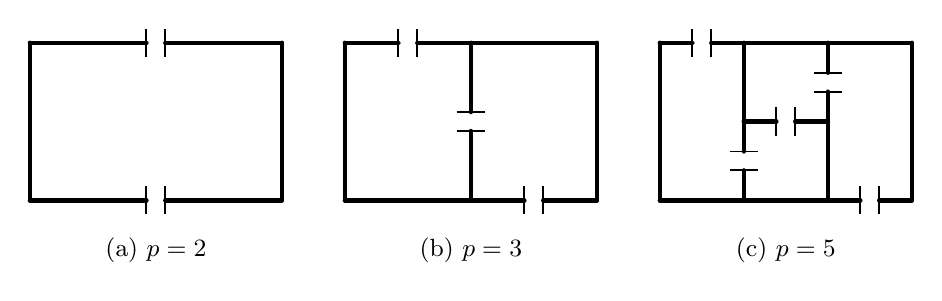
\begin{tikzpicture}[
			>=stealth, line width=0.8pt,
			trave/.style={line width=1.6pt, line cap=round,
				line join=round, black},
			taglio/.style={line width=0.7pt, black}]
			
			%% ===============================================================
			%% PANNELLO (a) — trave biconnessa: rettangolo (p = 2)
			%% ===============================================================
			\begin{scope}[xshift=0cm, yshift=0cm]
				
				\def\W{3.2}      %% larghezza del rettangolo
				\def\H{2.0}      %% altezza
				\def\dt{0.12}    %% mezza-larghezza dell'interruzione di trave
				\def\el{0.18}    %% mezza-lunghezza del trattino trasversale
				
				%% Posizione dei due tagli:
				%% uno sul lato superiore in W/2, uno sul lato inferiore in W/2
				\pgfmathsetmacro{\xTa}{\W*0.5}    %% taglio superiore
				\pgfmathsetmacro{\xTb}{\W*0.5}    %% taglio inferiore
				
				%% --- lato superiore: due segmenti, interrotto in xTa ---
				\draw[trave] (0,\H) -- ({\xTa-\dt},\H);
				\draw[trave] ({\xTa+\dt},\H) -- (\W,\H);
				%% trattini trasversali del taglio superiore
				\draw[taglio] ({\xTa-\dt},{\H-\el}) -- ({\xTa-\dt},{\H+\el});
				\draw[taglio] ({\xTa+\dt},{\H-\el}) -- ({\xTa+\dt},{\H+\el});
				
				%% --- lato inferiore: due segmenti, interrotto in xTb ---
				\draw[trave] (0,0) -- ({\xTb-\dt},0);
				\draw[trave] ({\xTb+\dt},0) -- (\W,0);
				%% trattini trasversali del taglio inferiore
				\draw[taglio] ({\xTb-\dt},{-\el}) -- ({\xTb-\dt},{\el});
				\draw[taglio] ({\xTb+\dt},{-\el}) -- ({\xTb+\dt},{\el});
				
				%% --- lati corti, integri ---
				\draw[trave] (0,0) -- (0,\H);
				\draw[trave] (\W,0) -- (\W,\H);
				
				%% --- etichetta pannello ---
				\node[below=10pt, font=\small] at (\W/2,0) {(a) $p=2$};
			\end{scope}
			
			%% ===============================================================
			%% PANNELLO (b) — triconnessa: + un setto verticale (p = 3)
			%% ===============================================================
			\begin{scope}[xshift=4cm, yshift=0cm]
				
				\def\W{3.2}      %% larghezza del rettangolo
				\def\H{2.0}      %% altezza
				\def\dt{0.12}    %% mezza-larghezza dell'interruzione
				\def\el{0.18}    %% mezza-lunghezza del trattino trasversale
				
				%% Posizione dei tre tagli
				\pgfmathsetmacro{\xTa}{\W*0.25}   %% sup, sinistra del setto
				\pgfmathsetmacro{\xTb}{\W*0.75}   %% inf, destra del setto
				\pgfmathsetmacro{\xS}{\W*0.50}    %% ascissa setto verticale
				\pgfmathsetmacro{\yTs}{\H*0.50}   %% taglio sul setto, a meta' altezza
				
				%% --- lato superiore: interrotto in xTa, setto in xS (continuo) ---
				\draw[trave] (0,\H) -- ({\xTa-\dt},\H);
				\draw[trave] ({\xTa+\dt},\H) -- (\W,\H);
				\draw[taglio] ({\xTa-\dt},{\H-\el}) -- ({\xTa-\dt},{\H+\el});
				\draw[taglio] ({\xTa+\dt},{\H-\el}) -- ({\xTa+\dt},{\H+\el});
				
				%% --- lato inferiore: interrotto in xTb ---
				\draw[trave] (0,0) -- ({\xTb-\dt},0);
				\draw[trave] ({\xTb+\dt},0) -- (\W,0);
				\draw[taglio] ({\xTb-\dt},{-\el}) -- ({\xTb-\dt},{\el});
				\draw[taglio] ({\xTb+\dt},{-\el}) -- ({\xTb+\dt},{\el});
				
				%% --- lati corti, integri ---
				\draw[trave] (0,0) -- (0,\H);
				\draw[trave] (\W,0) -- (\W,\H);
				
				%% --- setto verticale interno, interrotto in yTs ---
				\draw[trave] (\xS,0) -- (\xS,{\yTs-\dt});
				\draw[trave] (\xS,{\yTs+\dt}) -- (\xS,\H);
				%% trattini orizzontali del taglio sul setto
				\draw[taglio] ({\xS-\el},{\yTs-\dt}) -- ({\xS+\el},{\yTs-\dt});
				\draw[taglio] ({\xS-\el},{\yTs+\dt}) -- ({\xS+\el},{\yTs+\dt});
				
				%% --- etichetta pannello ---
				\node[below=10pt, font=\small] at (\W/2,0) {(b) $p=3$};
			\end{scope}
			
			%% ===============================================================
			%% PANNELLO (c) — p = 5: + due setti verticali + uno orizzontale
			%% ===============================================================
			\begin{scope}[xshift=8cm, yshift=0cm]
				
				\def\W{3.2}      %% larghezza del rettangolo
				\def\H{2.0}      %% altezza
				\def\dt{0.12}    %% mezza-larghezza dell'interruzione
				\def\el{0.18}    %% mezza-lunghezza del trattino trasversale
				
				%% Ascisse dei due setti verticali interni: in W/3 e 2W/3
				\pgfmathsetmacro{\xSa}{\W/3}      %% setto verticale sinistro
				\pgfmathsetmacro{\xSb}{2*\W/3}    %% setto verticale destro
				\pgfmathsetmacro{\yO}{\H*0.50}    %% quota del setto orizzontale
				
				%% Posizione dei cinque tagli
				\pgfmathsetmacro{\xTa}{\W/6}      %% taglio 1: sup, sx del setto sx
				\pgfmathsetmacro{\xTb}{5*\W/6}    %% taglio 2: inf, dx del setto dx
				\pgfmathsetmacro{\yTc}{\H*0.25}   %% taglio 3: setto sx, sotto
				\pgfmathsetmacro{\yTd}{\H*0.75}   %% taglio 4: setto dx, sopra
				\pgfmathsetmacro{\xTe}{\W*0.50}   %% taglio 5: setto orizz., centro
				
				%% --- lato superiore: interrotto in xTa, attraversato dai due setti ---
				\draw[trave] (0,\H) -- ({\xTa-\dt},\H);
				\draw[trave] ({\xTa+\dt},\H) -- (\W,\H);
				\draw[taglio] ({\xTa-\dt},{\H-\el}) -- ({\xTa-\dt},{\H+\el});
				\draw[taglio] ({\xTa+\dt},{\H-\el}) -- ({\xTa+\dt},{\H+\el});
				
				%% --- lato inferiore: interrotto in xTb ---
				\draw[trave] (0,0) -- ({\xTb-\dt},0);
				\draw[trave] ({\xTb+\dt},0) -- (\W,0);
				\draw[taglio] ({\xTb-\dt},{-\el}) -- ({\xTb-\dt},{\el});
				\draw[taglio] ({\xTb+\dt},{-\el}) -- ({\xTb+\dt},{\el});
				
				%% --- lati corti, integri ---
				\draw[trave] (0,0) -- (0,\H);
				\draw[trave] (\W,0) -- (\W,\H);
				
				%% --- setto verticale sx: interrotto in yTc (sotto) ---
				\draw[trave] (\xSa,0) -- (\xSa,{\yTc-\dt});
				\draw[trave] (\xSa,{\yTc+\dt}) -- (\xSa,\H);
				\draw[taglio] ({\xSa-\el},{\yTc-\dt}) -- ({\xSa+\el},{\yTc-\dt});
				\draw[taglio] ({\xSa-\el},{\yTc+\dt}) -- ({\xSa+\el},{\yTc+\dt});
				
				%% --- setto verticale dx: interrotto in yTd (sopra) ---
				\draw[trave] (\xSb,0) -- (\xSb,{\yTd-\dt});
				\draw[trave] (\xSb,{\yTd+\dt}) -- (\xSb,\H);
				\draw[taglio] ({\xSb-\el},{\yTd-\dt}) -- ({\xSb+\el},{\yTd-\dt});
				\draw[taglio] ({\xSb-\el},{\yTd+\dt}) -- ({\xSb+\el},{\yTd+\dt});
				
				%% --- setto orizzontale: da xSa a xSb, interrotto in xTe ---
				\draw[trave] (\xSa,\yO) -- ({\xTe-\dt},\yO);
				\draw[trave] ({\xTe+\dt},\yO) -- (\xSb,\yO);
				\draw[taglio] ({\xTe-\dt},{\yO-\el}) -- ({\xTe-\dt},{\yO+\el});
				\draw[taglio] ({\xTe+\dt},{\yO-\el}) -- ({\xTe+\dt},{\yO+\el});
				
				%% --- etichetta pannello ---
				\node[below=10pt, font=\small] at (\W/2,0) {(c) $p=5$};
			\end{scope}
			
		\end{tikzpicture}
	}
	\caption{Travi pluriconnesse di grado crescente. In
		ciascun pannello i $p$ tagli trasversali necessari
		a separare la linea d'asse in due tratti
		monoconnessi sono indicati dall'interruzione della
		linea fra due trattini paralleli.
		(a)~Trave biconnessa ($p = 2$): la linea
		d'asse è chiusa; due tagli la separano in due
		tratti monoconnessi. L'iperstaticità interna è
		$3(p-1) = 3$.
		(b)~Trave triconnessa ($p = 3$): un setto
		verticale interno introduce un secondo anello;
		tre tagli separano la trave in due tratti
		monoconnessi. L'iperstaticità interna è
		$3(p-1) = 6$.
		(c)~Trave pluriconnessa con $p = 5$: due setti
		verticali interni e un setto orizzontale corto
		che li collega creano quattro anelli; cinque
		tagli separano la trave in due tratti monoconnessi.
		L'iperstaticità interna è $3(p-1) = 12$.
		Il grado di connessione dipende solo dalla
		topologia della linea d'asse, indipendentemente
		dai vincoli esterni (qui assenti).}
	\label{fig:gradi_connessione}
\end{figure}




\begin{oss}
	Il grado di connessione $p$ è un invariante
	topologico: non dipende dalla forma della linea
	d'asse né dalla posizione dei vincoli, ma solo
	dal numero di ``anelli'' presenti nella geometria
	della trave. Una trave rettilinea, una trave
	ad arco e una trave a L sono tutte monoconnesse;
	una trave ad anello circolare o rettangolare è
	biconnessa.
\end{oss}

%----------------------------------------------------------------------------------------------------------------------------
\subsection{Iperstaticità interna delle travi pluriconnesse}
\label{sec:ipestat_interna}
%----------------------------------------------------------------------------------------------------------------------------

La trave pluriconnessa di grado $p$ è
\emph{internamente iperstatica}\index{iperstaticita@iperstaticità!interna|textbf} di grado $3(p-1)$:
i $p-1$ tagli necessari a renderla aperta
introducono $3(p-1)$ incognite statiche aggiuntive
--- le caratteristiche della sollecitazione nelle
$p-1$ sezioni di taglio --- che non sono
determinabili dalle sole equazioni di equilibrio.


Per comprendere perché, consideriamo una trave
biconnessa ($p = 2$): la linea d'asse è chiusa
e un solo taglio in $S$ la rende aperta. Il sistema
dopo il taglio ha ancora $n_c = 1$ corpo --- la
trave resa aperta --- con $n = 3$ incognite
cinematiche e $m_{\rm est}$ vincoli esterni, ai
quali si aggiungono le \emph{condizioni di chiusura
	dell'anello}\index{condizioni di chiusura dell'anello|textbf} sul versante cinematico e le
caratteristiche della sollecitazione $N(S)$, $T(S)$,
$M(S)$ sul versante statico.

Le tre condizioni di chiusura dell'anello impongono
che lo spostamento assiale $w$, lo spostamento
longitudinale $v$ e la rotazione $\vartheta$ assumano
lo stesso valore alle due facce $S^-$ ed $S^+$
della sezione di taglio. Sono le tre condizioni
cinematiche del vincolo di rigidità in $S$,
applicate alla configurazione chiusa dell'anello:
senza di esse l'anello si ``aprirebbe'' in
corrispondenza di $S$.

\paragraph{Problema cinematico.}
Le $3$ condizioni di chiusura dell'anello
costituiscono $3$ equazioni di vincolo aggiuntive
sulle $3$ incognite cinematiche della trave aperta.
Il numero nominale di gradi di libertà diventa:
\begin{equation}
	\nu = 3 - (m_{\rm est} + 3)
	= (3 - m_{\rm est}) - 3
	= \nu_{\rm aperta} - 3,
\end{equation}
dove $\nu_{\rm aperta} = 3 - m_{\rm est}$ è il
numero nominale della trave resa aperta. Se la
trave aperta è isostatica ($\nu_{\rm aperta} = 0$),
la trave chiusa ha $\nu = -3$: è iperstatica di
grado $3 = 3(p-1)$, coerentemente con la formula
generale.

Le condizioni di chiusura dell'anello sono
\emph{condizioni di compatibilità cinematica}:
non è possibile assegnare distorsioni arbitrarie
nella sezione di taglio senza violare la chiusura
geometrica dell'anello. Le distorsioni ammissibili
devono soddisfare $3(p-1)$ condizioni di
compatibilità --- l'analogo delle condizioni
$\bm{R}_\chi^\top \bm{s} = \bm{0}$ del
\CAPref{cap:problemi_cin_stat_SCR} --- che
esprimono appunto la chiusura geometrica.
Questo vincolo non esiste per le travi monoconnesse,
dove le distorsioni possono essere assegnate
liberamente in qualsiasi sezione.


\paragraph{Problema statico.}
Le $3$ incognite statiche $N(S)$, $T(S)$, $M(S)$
non sono determinabili dalle sole equazioni di
equilibrio: il taglio introduce $3$ nuove incognite
senza aggiungere nuove equazioni --- le equazioni
di equilibrio della trave aperta sono le stesse di
prima del taglio. Il problema statico diventa quindi
indeterminato di grado $3 = 3(p-1)$, e le
caratteristiche della sollecitazione nella sezione
di taglio rimangono libere fino a che non si
introduce la legge costitutiva della trave
deformabile (Volume~II).



\begin{oss}
	L'iperstaticità interna delle travi pluriconnesse
	non dipende dai vincoli esterni: è una proprietà
	della sola geometria della linea d'asse. Una
	trave ad anello libera nello spazio --- senza
	alcun vincolo esterno --- è già internamente
	iperstatica di grado $3$: le tre caratteristiche
	della sollecitazione nella sezione di taglio
	non sono determinabili dall'equilibrio esterno,
	e le distorsioni in quella sezione non sono
	assegnabili liberamente senza verificare la
	compatibilità cinematica.
\end{oss}

\begin{oss}[Dualità cinematico-statica nelle travi	pluriconnesse]
	L'iperstaticità interna $3(p-1)$ è la manifestazione
	diretta della struttura duale $\bm{B} = \bm{A}^{\top}$
	applicata alla trave pluriconnessa. La
	\FIGref{fig:biconnessa_dualita} illustra il caso
	$p = 2$ (anello): nel versante cinematico le tre
	distorsioni $\varrho_w$, $\varrho_v$,
	$\varrho_\vartheta$ in $S$ rappresentano gli scarti
	cinematici fra le due facce della sezione di taglio
	e sono vincolate dalle tre condizioni di compatibilità
	$\varrho_w = \varrho_v = \varrho_\vartheta = 0$
	imposte dalla chiusura dell'anello; specularmente,
	sul versante statico le tre caratteristiche $N(S)$,
	$T(S)$, $M(S)$ agiscono sulle stesse facce come
	coppie autoequilibrate e restano indeterminate dalle
	sole equazioni di equilibrio.
	
	\begin{figure}[!htbp]
		\centering
		%\resizebox{\textwidth}{!}{%
			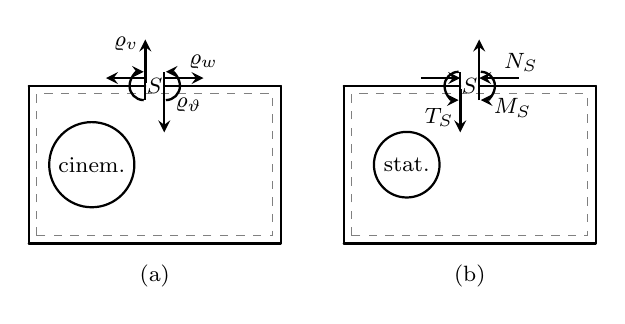
\begin{tikzpicture}[
				>=stealth, line width=0.8pt,
				trave/.style={line width=0.80pt, line cap=round, line join=round, black},
				taglio/.style={line width=0.8pt, black},    
				distor/.style={->, >=stealth, line width=0.9pt, black},
				sollec/.style={->, >=stealth, line width=0.9pt, black},
				etichetta/.style={circle, draw=black, inner sep=2.5pt,	line width=0.8pt, font=\footnotesize}]
				
				%% ===============================================================
				%% PANNELLO (a) — cinematico: tre distorsioni in S
				%% ===============================================================
				\begin{scope}[xshift=0cm, yshift=0cm]
					
					\def\W{3.2}
					\def\H{2.0}
					\def\dt{0.12}      %% mezza-larghezza dell'interruzione
					\def\el{0.18}      %% mezza-lunghezza del trattino trasversale
					
					\pgfmathsetmacro{\xS}{\W*0.5}      %% ascissa del taglio
					
					%% --- rettangolo con lato superiore interrotto in xS ---
					\draw[trave] (0,\H) -- ({\xS-\dt},\H);     %% lato sup. sinistro
					\draw[trave] ({\xS+\dt},\H) -- (\W,\H);    %% lato sup. destro
					\draw[trave] (0,0) -- (\W,0);              %% lato inferiore
					\draw[trave] (0,0) -- (0,\H);              %% lato sinistro
					\draw[trave] (\W,0) -- (\W,\H);            %% lato destro
					
					%% tratteggio della fibra inferiore: lato interno dell'anello
					\def\df{0.10}      %% distanza del tratteggio dal lato della trave
					\draw[dashed, thin, gray]
					({\df},{\df}) rectangle ({\W-\df},{\H-\df});
					
					%% --- trattini trasversali del taglio ---
					\draw[taglio] ({\xS-\dt},{\H-\el}) -- ({\xS-\dt},{\H+\el});
					\draw[taglio] ({\xS+\dt},{\H-\el}) -- ({\xS+\dt},{\H+\el});
					
					%% --- etichetta S in alto a destra del taglio ---
					\node[font=\footnotesize] at (\xS,\H) {$S$};
					
					%% --- varrho_w: due frecce orizzontali antagoniste SOPRA la trave ---
					%% (assiale: si avvicinano alle due facce dall'esterno)
					\pgfmathsetmacro{\yw}{\H+0.10}
					\def\dw{0.50}
					\draw[distor] (\xS-\dt,\yw) -- (\xS-\dw-\dt,\yw);
					\draw[distor] (\xS+\dt,\yw) -- (\xS+\dw+\dt,\yw);
					\node[font=\footnotesize, right=3pt] at (\xS+0.2,\yw+0.2)	{$\varrho_w$};
					
					%% --- varrho_v: due frecce verticali antagoniste,
					%%     attaccate agli estremi delle due facce ---
					%% (trasversale: una faccia scende, l'altra sale)
					\def\dv{0.55}
					\def\gv{0.04}      %% gap fra trattino-faccia e inizio freccia
					%% sulla faccia S^- (a sinistra del taglio): freccia verso l'alto
					\draw[distor] ({\xS-\dt},{\H+\gv}) -- ({\xS-\dt},{\H+\gv+\dv});
					%% sulla faccia S^+ (a destra del taglio): freccia verso il basso
					\draw[distor] ({\xS+\dt},{\H-\gv}) -- ({\xS+\dt},{\H-\gv-\dv});
					\node[font=\footnotesize, right=2pt] at ({\xS-\dt-0.6},{\H+\gv+\dv*0.9}) {$\varrho_v$};
					
					%% --- varrho_vartheta: due semiarchi antagonisti, sopra le facce ---
					\pgfmathsetmacro{\ya}{\H}      %% centro dei semiarchi
					\draw[->, >=stealth, line width=0.85pt]
					({\xS-0.14},{\ya-0.18}) arc (270:90:0.18);
					\draw[->, >=stealth, line width=0.85pt]	({\xS+0.14},{\ya-0.18}) arc (-90:90:0.18);
					\node[font=\footnotesize, right=1pt] at ({\xS+0.10},\ya-0.24) {$\varrho_\vartheta$};
					
					%% --- etichetta diagramma (in angolo interno dell'anello) ---
					\node[etichetta] at (\W*0.25,\H*0.5) {cinem.};
					
					%% --- etichetta pannello ---
					\node[below=4pt, font=\footnotesize] at (\W/2,0) {(a)};
				\end{scope}
				
				%% ===============================================================
				%% PANNELLO (b) — statico: tre caratteristiche in S come coppie
				%%                autoequilibrate, parametricamente libere
				%% ===============================================================
				\begin{scope}[xshift=4cm, yshift=0cm]
					
					\def\W{3.2}
					\def\H{2.0}
					\def\dt{0.12}      %% mezza-larghezza dell'interruzione
					\def\el{0.18}      %% mezza-lunghezza del trattino trasversale
					
					\pgfmathsetmacro{\xS}{\W*0.5}      %% ascissa del taglio
					
					%% --- rettangolo con lato superiore interrotto in xS ---
					\draw[trave] (0,\H) -- ({\xS-\dt},\H);     %% lato sup. sinistro
					\draw[trave] ({\xS+\dt},\H) -- (\W,\H);    %% lato sup. destro
					\draw[trave] (0,0) -- (\W,0);              %% lato inferiore
					\draw[trave] (0,0) -- (0,\H);              %% lato sinistro
					\draw[trave] (\W,0) -- (\W,\H);            %% lato destro
					
					%% tratteggio della fibra inferiore: lato interno dell'anello
					\def\df{0.10}      %% distanza del tratteggio dal lato della trave
					\draw[dashed, thin, gray]
					({\df},{\df}) rectangle ({\W-\df},{\H-\df});
					
					
					%% --- trattini trasversali del taglio ---
					\draw[taglio] ({\xS-\dt},{\H-\el}) -- ({\xS-\dt},{\H+\el});
					\draw[taglio] ({\xS+\dt},{\H-\el}) -- ({\xS+\dt},{\H+\el});
					
					%% --- etichetta S in alto a destra del taglio ---
					\node[font=\footnotesize] at (\xS,\H) {$S$};
					
					%% --- varrho_w: due frecce orizzontali antagoniste SOPRA la trave ---
					%% (assiale: si avvicinano alle due facce dall'esterno)
					\pgfmathsetmacro{\yw}{\H+0.10}
					\def\dw{0.50}
					\draw[distor] (\xS-\dw-\dt,\yw) -- (\xS-\dt,\yw);
					\draw[distor] (\xS+\dw+\dt,\yw) -- (\xS+\dt,\yw);
					\node[font=\footnotesize, right=3pt] at (\xS+0.2,\yw+0.2)	{$N_S$};
					
					%% --- T_S due frecce verticali antagoniste,
					%%     attaccate agli estremi delle due facce ---
					%% (trasversale: una faccia scende, l'altra sale)
					\def\dv{0.55}
					\def\gv{0.04}      %% gap fra trattino-faccia e inizio freccia
					\draw[distor] ({\xS-\dt},{\H-\gv}) -- ({\xS-\dt},{\H-\gv-\dv});
					\draw[distor] ({\xS+\dt},{\H+\gv}) -- ({\xS+\dt},{\H+\gv+\dv});
					%\draw[distor] ({\xS+\dt},{\H-\gv}) -- ({\xS+\dt},{\H-\gv-\dv});
					\node[font=\footnotesize, right=2pt] at ({\xS-\dt-0.65},{\H+\gv-\dv*0.8}) {$T_S$};
					
					%% --- M_S: due semiarchi antagonisti, ---
					\pgfmathsetmacro{\ya}{\H}      %% centro dei semiarchi
					\draw[<-, >=stealth, line width=0.85pt]	({\xS-0.14},{\ya-0.18}) arc (270:90:0.18);
					\draw[<-, >=stealth, line width=0.85pt]	({\xS+0.14},{\ya-0.18}) arc (-90:90:0.18);
					\node[font=\footnotesize, right=1pt] at ({\xS+0.14},\ya-0.28) {$M_S$};
					
					%% --- etichetta diagramma (in angolo interno dell'anello) ---
					\node[etichetta] at (\W*0.25,\H*0.5) {stat.};
					
					%% --- etichetta pannello ---
					\node[below=4pt, font=\footnotesize] at (\W/2,0) {(b)};
				\end{scope}
				
			\end{tikzpicture}%
			%}%
		\caption{Trave biconnessa con taglio ideale in $S$:
			rappresentazione duale delle tre grandezze cinematiche
			e statiche associate al vincolo di rigidità.
			(a)~Le tre distorsioni $\varrho_w$, $\varrho_v$,
			$\varrho_\vartheta$ come scarti cinematici fra le
			due facce $S^-$ ed $S^+$.
			(b)~Le tre caratteristiche della sollecitazione
			$N(S)$, $T(S)$, $M(S)$ come azioni interne agenti
			sulle stesse facce. Le grandezze sono disegnate nel
			verso positivo secondo le convenzioni di segno}
		\label{fig:biconnessa_dualita}
	\end{figure}
	
	La corrispondenza è biunivoca: a ciascuna condizione
	di compatibilità cinematica nel pannello~(a)
	corrisponde un'incognita statica nel pannello~(b).
	Il caso generale $p \geq 2$ replica la stessa
	struttura su ciascuno dei $p-1$ tagli necessari ad
	aprire la linea d'asse, da cui l'iperstaticità di
	grado $3(p-1)$.
\end{oss}



%----------------------------------------------------------------------------------------------------------------------------
\subsection{Svincoli interni}
\label{sec:svincoli_interni}
%----------------------------------------------------------------------------------------------------------------------------

Indipendentemente dal grado di connessione, è possibile
introdurre degli \emph{svincoli}\index{svincolo!interno} in una o più zone di
connessione della trave: rilasci parziali del vincolo
di rigidità che riducono il numero di condizioni
cinematiche attive e, dualmente, il numero di
caratteristiche della sollecitazione trasmesse
attraverso la zona di connessione.

Nel riferimento intrinseco $(O^e;\, y^e,\, z^e)$ il
vincolo di rigidità impone in $S$ le tre condizioni
\[
\llbracket w \rrbracket_S = 0, \qquad
\llbracket v \rrbracket_S = 0, \qquad
\llbracket \vartheta \rrbracket_S = 0,
\]
cui corrispondono dualmente le tre caratteristiche
della sollecitazione $N$, $T$, $M$. In base al numero
di condizioni rilasciate, gli svincoli si classificano
in:
\begin{itemize}[nosep]
	\item \emph{svincoli semplici}\index{svincolo!semplice|textbf}, che rilasciano una
	sola delle tre condizioni;
	\item \emph{svincoli multipli}\index{svincolo!multiplo|textbf}, che ne rilasciano
	due simultaneamente.
\end{itemize}
Il rilascio di tutte e tre le condizioni equivale a una
\emph{sconnessione completa} fra i due tratti --- la
zona di connessione viene rimossa --- e non figura nel
catalogo degli svincoli.

\paragraph{Svincoli semplici.}
Si distinguono in tre tipi, secondo la condizione
rilasciata:
\begin{itemize}[nosep]
	\item \textbf{svincolo rotazionale}\index{svincolo!rotazionale|textbf}: rilascia la
	condizione $\llbracket\vartheta\rrbracket_S = 0$,
	lasciando libera la rotazione relativa fra i due
	tratti. Il momento flettente $M$ non viene più
	trasmesso attraverso la zona di connessione. Il
	dispositivo meccanico corrispondente è la
	\emph{cerniera interna}\index{cerniera!interna};
	\item \textbf{svincolo traslazionale in $y^e$}\index{svincolo!traslazionale|textbf}:
	rilascia la condizione $\llbracket v \rrbracket_S = 0$,
	lasciando libero lo scorrimento relativo trasversale.
	Il taglio $T$ non viene più trasmesso. Il dispositivo
	meccanico corrispondente è il \emph{glifo interno
		con asse $z^e$};
	\item \textbf{svincolo traslazionale in $z^e$}:
	rilascia la condizione $\llbracket w \rrbracket_S = 0$,
	lasciando libero lo scorrimento relativo assiale.
	La forza normale $N$ non viene più trasmessa. Il
	dispositivo meccanico corrispondente è il
	\emph{glifo interno con asse $y^e$}.
\end{itemize}

\paragraph{Svincoli multipli.}
La composizione di due svincoli semplici nella stessa
zona di connessione rilascia due delle tre condizioni
di rigidità: ne resta attiva una sola e, dualmente, una
sola caratteristica della sollecitazione viene
trasmessa attraverso $S$. Le combinazioni indipendenti
sono tre:
\begin{itemize}[nosep]
	\item \textbf{biella longitudinale}\index{biella!longitudinale|textbf}: rilascia
	$\llbracket v\rrbracket_S = 0$ e
	$\llbracket\vartheta\rrbracket_S = 0$; resta attiva
	la sola continuità assiale
	$\llbracket w\rrbracket_S = 0$ e si trasmette la
	sola forza normale $N$;
	\item \textbf{biella trasversale}\index{biella!trasversale|textbf}: rilascia
	$\llbracket w\rrbracket_S = 0$ e
	$\llbracket\vartheta\rrbracket_S = 0$; resta attiva
	la sola continuità trasversale
	$\llbracket v\rrbracket_S = 0$ e si trasmette il
	solo taglio $T$;
	\item \textbf{bipendolo interno}\index{bipendolo!interno}: rilascia
	$\llbracket w\rrbracket_S = 0$ e
	$\llbracket v\rrbracket_S = 0$; resta attiva la
	sola continuità rotazionale
	$\llbracket\vartheta\rrbracket_S = 0$ e si trasmette
	il solo momento flettente $M$.
\end{itemize}

\paragraph{Catalogo sistematico.}
I sei dispositivi --- tre semplici e tre multipli ---
sono raccolti nella Tabella~\ref{tab:svincoli_interni},
organizzata in due blocchi separati da un filetto
doppio. Per ciascuna riga, la colonna centrale riporta
le condizioni cinematiche \emph{attive} attraverso $S$
(quelle \emph{non} rilasciate dallo svincolo) e la
colonna destra le caratteristiche della sollecitazione
\emph{trasmesse}. La decodifica si fonda sulla
corrispondenza biunivoca
\[
\llbracket w\rrbracket_S \;\longleftrightarrow\; N,
\qquad
\llbracket v\rrbracket_S \;\longleftrightarrow\; T,
\qquad
\llbracket\vartheta\rrbracket_S \;\longleftrightarrow\; M,
\]
e sulla \emph{regola di complementarità}\index{regola di complementarita@regola di complementarità}: il numero di
condizioni cinematiche attive e quello delle
caratteristiche trasmesse hanno per somma tre, pari al
numero di condizioni imposte dal vincolo di rigidità.


\begin{table}[!htbp]
	\centering
	\caption{Svincoli interni della trave rigida: catalogo
		sistematico. Ciascuno svincolo rilascia una o più
		delle tre condizioni del vincolo di rigidità in $S$,
		lasciando attive le rimanenti e, per dualità, le
		caratteristiche della sollecitazione corrispondenti.}
	\label{tab:svincoli_interni}
	\begin{tabular}{@{}>{\centering\arraybackslash}m{4.0cm}
			>{\centering\arraybackslash}m{4.5cm}
			>{\centering\arraybackslash}m{3cm}@{}}
		\toprule
		\textbf{Dispositivo} 
		& \shortstack{\textbf{Condizioni}\\\textbf{cinematiche attive}}	& \shortstack{\textbf{Caratteristiche}\\\textbf{trasmesse}} \\
		\midrule
		%% --- SVINCOLI SEMPLICI ---
		%% cella cerniera 
		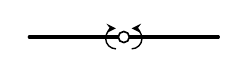
\begin{tikzpicture}[
			>=stealth, line width=0.6pt,
			trave/.style={line width=1.2pt, line cap=round,
				line join=round, black},
			nodoV/.style={circle, fill=white, draw=black,
				inner sep=0pt, minimum size=4pt,
				line width=0.6pt}]
			\def\W{2.4}
			\pgfmathsetmacro{\xS}{\W*0.5}
			
			%% trave continua
			\draw[trave] (0,0) -- (\W,0);
			
			%% cerniera interna
			\node[nodoV] at (\xS,0) {};
			
			%% moto relativo rilasciato: arco varrho_vartheta
			\pgfmathsetmacro{\ya}{0.35}
			\draw[->, >=stealth, line width=0.5pt]	({\xS-0.10},{\ya-0.50}) arc (270:90:0.13);
			\draw[->, >=stealth, line width=0.5pt]	({\xS+0.10},{\ya-0.50}) arc (-90:90:0.13);
		\end{tikzpicture}
		& $\llbracket w \rrbracket_S = 0$, $\llbracket v \rrbracket_S = 0$
		& $N$, $T$ \\
		\midrule
		%% glifo asse z^e
		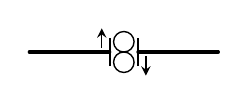
\begin{tikzpicture}[
			>=stealth, line width=0.6pt, trave/.style={line width=1.2pt, line cap=round, line join=round, black}]
			\def\W{2.4}
			\pgfmathsetmacro{\xS}{\W*0.5}
			
			%% trave interrotta, piatti verticali alle estremità
			\def\dt{0.18}    %% mezza-larghezza dell'interruzione
			\def\hp{0.18}    %% mezza-altezza dei piatti
			\draw[trave] (0,0) -- (\xS-\dt,0);
			\draw[trave] (\xS+\dt,0) -- (\W,0);
			\draw[line width=0.8pt] (\xS-\dt,-\hp) -- (\xS-\dt,\hp);
			\draw[line width=0.8pt] (\xS+\dt,-\hp) -- (\xS+\dt,\hp);
			
			%% due rotelle tangenti ai piatti
			\pgfmathsetmacro{\r}{\dt-0.05}
			\draw[line width=0.5pt] (\xS,\r) circle (\r);
			\draw[line width=0.5pt] (\xS,-\r) circle (\r);
			
			%% frecce del moto relativo rilasciato
			\draw[->, line width=0.5pt] ({\xS-\dt-0.1},0.05) -- ({\xS-\dt-0.1},0.30);
			\draw[->, line width=0.5pt] ({\xS+\dt+0.1},-0.05) -- ({\xS+\dt+0.1},-0.30);
		\end{tikzpicture}
		& $\llbracket w \rrbracket_S = 0$, $\llbracket \vartheta \rrbracket_S = 0$
		& $N$, $M$ \\
		\midrule
	
		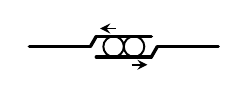
\begin{tikzpicture}[
			>=stealth, line width=0.8pt,
			trave/.style={line width=1.2pt, line cap=round,	line join=round, black}, ruota/.style={line width=0.7pt, black},
			moto/.style={->, >=stealth, line width=0.6pt, black}]
			
			\def\W{2.4}
			\pgfmathsetmacro{\xS}{\W*0.5}
			
			\def\r{0.13}                       %% raggio delle rotelle
			\pgfmathsetmacro{\dx}{\r/tan(60)}  %% spostamento orizz. della deviazione
			%% Punti chiave (tronco sinistro)
			\pgfmathsetmacro{\xA}{\xS-0.35-\dx}  %% inizio deviazione sx
			\pgfmathsetmacro{\xB}{\xS-0.35}      %% fine deviazione sx
			\pgfmathsetmacro{\xC}{\xS+0.35}      %% fine prolungamento sx
			%% Punti speculari (tronco destro)
			\pgfmathsetmacro{\xD}{\xS+0.35+\dx}  %% inizio deviazione dx
			
			%% --- tronco sinistro: trave → deviazione → prolungamento ---
			\draw[trave] (0,0) -- (\xA,0);
			\draw[trave] (\xA,0) -- (\xB,\r);
			\draw[trave] (\xB,\r) -- (\xC,\r);
			
			%% --- tronco destro (speculare) ---
			\draw[trave] (\xD,0) -- (\W,0);
			\draw[trave] (\xD,0) -- (\xC,-\r);
			\draw[trave] (\xC,-\r) -- (\xB,-\r);
			
			%% --- due rotelle tangenti ai due prolungamenti ---
			\draw[ruota] (\xS-\r,0) circle (\r);
			\draw[ruota] (\xS+\r,0) circle (\r);
			
			%% --- frecce del moto relativo rilasciato (varrho_w longitudinale) ---
			%% sul prolungamento sx (sopra): freccia verso sinistra
			\pgfmathsetmacro{\xfreccia}{\xB+0.05}
			\pgfmathsetmacro{\yfreccia}{\r+0.10}
			\draw[moto] (\xfreccia+0.20,\yfreccia) -- (\xfreccia,\yfreccia);
			%% sul prolungamento dx (sotto): freccia verso destra
			\draw[moto] (\xC-0.05-0.20,-\yfreccia) -- (\xC-0.05,-\yfreccia);
			
			%% --- etichetta S sotto la trave (lontano dal dispositivo) ---
			%\node[font=\footnotesize, below=8pt] at (\xS,-\r) {$S$};
			
		\end{tikzpicture}
		& $\llbracket v \rrbracket_S = 0$, $\llbracket \vartheta \rrbracket_S = 0$
		& $T$, $M$ \\
		\midrule\midrule    %% doppia linea: passaggio a svincoli multipli
		%% --- SVINCOLI MULTIPLI ---
		%% biella longitudinale
		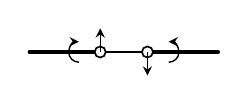
\begin{tikzpicture}[
			>=stealth, line width=0.6pt,
			trave/.style={line width=1.2pt, line cap=round,
				line join=round, black},
			nodoV/.style={circle, fill=white, draw=black,
				inner sep=0pt, minimum size=4pt,
				line width=0.6pt},
			moto/.style={->, >=stealth, line width=0.5pt, black}]
			
			\def\W{2.4}
			\pgfmathsetmacro{\xS}{\W*0.5}
			
			%% trave interrotta
			\def\dt{0.30}
			\draw[trave] (0,0) -- (\xS-\dt,0);
			\draw[trave] (\xS+\dt,0) -- (\W,0);
			
			%% biella longitudinale: segmento + due perni
			\draw[line width=0.8pt] (\xS-\dt,0) -- (\xS+\dt,0);
			\node[nodoV] at (\xS-\dt,0) {};
			\node[nodoV] at (\xS+\dt,0) {};
			
			%% frecce dei due moti rilasciati:
			%% (1) scorrimento trasversale: due frecce verticali antagoniste,
			%%     in asse alle due cerniere (coda nella cerniera)
			\draw[moto] (\xS-\dt,0) -- (\xS-\dt,0.30);    %% sx: verso l'alto
			\draw[moto] (\xS+\dt,0) -- (\xS+\dt,-0.30);   %% dx: verso il basso
			
			%% (2) rotazione relativa: due semicirconferenze antagoniste,
			%%     a sinistra e a destra del dispositivo
			\draw[moto] ({\xS-\dt-0.27},-0.13) arc (270:90:0.13);   %% sx
			\draw[moto] ({\xS+\dt+0.27},-0.13) arc (-90:90:0.13);   %% dx
			
			
		\end{tikzpicture}
		& $\llbracket w \rrbracket_S = 0$
		& $N$ \\
		\midrule
		%% biella trasversale
		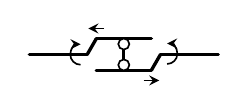
\begin{tikzpicture}[
			>=stealth, line width=0.8pt,
			trave/.style={line width=1.2pt, line cap=round,	line join=round, black},
			biella/.style={line width=1.0pt, black},
			nodoV/.style={circle, fill=white, draw=black,
				inner sep=0pt, minimum size=4pt,
				line width=0.6pt},
			moto/.style={->, >=stealth, line width=0.6pt, black}]
			
			\def\W{2.4}
			\pgfmathsetmacro{\xS}{\W*0.5}
			
			\def\r{0.20}                       %% mezza-lunghezza biella verticale
			\pgfmathsetmacro{\dx}{\r/tan(60)}  %% spostamento orizz. deviazione
			\pgfmathsetmacro{\xA}{\xS-0.35-\dx}  %% inizio deviazione sx
			\pgfmathsetmacro{\xB}{\xS-0.35}      %% fine deviazione sx
			\pgfmathsetmacro{\xC}{\xS+0.35}      %% fine prolungamento sx
			\pgfmathsetmacro{\xD}{\xS+0.35+\dx}  %% inizio deviazione dx
			
			%% --- tronco sinistro: trave -> deviazione -> prolungamento sopra ---
			\draw[trave] (0,0) -- (\xA,0);
			\draw[trave] (\xA,0) -- (\xB,\r);
			\draw[trave] (\xB,\r) -- (\xC,\r);
			
			%% --- tronco destro (speculare, prolungamento sotto) ---
			\draw[trave] (\xD,0) -- (\W,0);
			\draw[trave] (\xD,0) -- (\xC,-\r);
			\draw[trave] (\xC,-\r) -- (\xB,-\r);
			
			
			\def\rp{0.067}    %% raggio del nodoV (minimum size=4pt ≈ 0.067 in coord. tikz)
			\pgfmathsetmacro{\yPsup}{\r-\rp}    %% centro perno superiore
			\pgfmathsetmacro{\yPinf}{-\r+\rp}   %% centro perno inferiore
			\draw[biella] (\xS,\yPsup) -- (\xS,\yPinf);
			\node[nodoV] at (\xS,\yPsup) {};
			\node[nodoV] at (\xS,\yPinf) {};
			
			%% --- frecce dei due moti rilasciati ---
			%% (1) scorrimento longitudinale: due frecce orizzontali antagoniste
			%%     sui prolungamenti, in asse alla biella
			\pgfmathsetmacro{\yfa}{\r+0.13}
			\draw[moto] (\xB+0.10,\yfa) -- (\xB-0.10,\yfa);    %% sx verso sin.
			\draw[moto] (\xC-0.10,-\yfa) -- (\xC+0.10,-\yfa);  %% dx verso des.
			
			%% (2) rotazione relativa: due semicirconferenze antagoniste
			%%     sopra e sotto la biella, da una parte e dall'altra
			\draw[moto] ({\xB-0.20},{\r-0.33}) arc (270:90:0.13);    %% sx
			\draw[moto] ({\xC+0.20},{-\r+0.08}) arc (-90:90:0.13);   %% dx
			
			%% --- etichetta S ---
			%\node[font=\footnotesize, below=8pt] at (\xS,-\r) {$S$};
			
		\end{tikzpicture}
		& $\llbracket v \rrbracket_S = 0$
		& $T$ \\
		\midrule
		%% bipendolo interno
		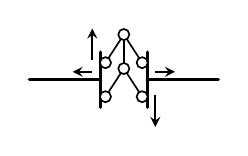
\begin{tikzpicture}[
			>=stealth, line width=0.8pt,
			trave/.style={line width=1.2pt, line cap=round,
				line join=round, black},
			asta/.style={line width=0.6pt, black},
			biella/.style={line width=0.6pt, black},
			nodoV/.style={circle, fill=white, draw=black,
				inner sep=0pt, minimum size=4pt,
				line width=0.6pt},
			moto/.style={->, >=stealth, line width=0.6pt, black}]
			
			\def\W{2.40}
			\pgfmathsetmacro{\xS}{\W*0.5}
			
			
			\def\d{0.30}                       %% mezza-distanza fra i piatti (allargata)
			\def\h{0.35}                       %% mezza-altezza piatti
			
			\def\rp{0.067}                     %% raggio dei perni nodoV
			\def\angle{50}                     %% inclinazione aste
			
			%% Quote dei perni: interne al piatto
			\pgfmathsetmacro{\yP}{\h-2*\rp}    %% 0.166
			
			%% Ascisse dei perni: tangenti dall'interno (perni dentro al dispositivo)
			\pgfmathsetmacro{\xPsx}{\xS-\d+\rp}   %% bordo sx del perno tocca il piatto sx
			\pgfmathsetmacro{\xPdx}{\xS+\d-\rp}   %% bordo dx del perno tocca il piatto dx
			
			\pgfmathsetmacro{\dy}{\d*tan(\angle)}
			\pgfmathsetmacro{\yPa}{\yP+\dy}    %% P_A sopra
			\pgfmathsetmacro{\yPb}{-\yP+\dy}   %% P_B poco sopra la trave
			
			%% --- tronchi di trave ---
			\draw[trave] (0,0) -- (\xS-\d,0);
			\draw[trave] (\xS+\d,0) -- (\W,0);
			
			%% --- piatti trasversali (spessi come la trave) ---
			\draw[trave] (\xS-\d,-\h) -- (\xS-\d,\h);
			\draw[trave] (\xS+\d,-\h) -- (\xS+\d,\h);
			
			%% --- 4 aste: dai perni interni tangenti ai piatti ---
			\draw[asta] (\xPsx,\yP)   -- (\xS,\yPa);
			\draw[asta] (\xPsx,-\yP)  -- (\xS,\yPb);
			\draw[asta] (\xPdx,\yP)   -- (\xS,\yPa);
			\draw[asta] (\xPdx,-\yP)  -- (\xS,\yPb);
			
			%% --- biella verticale centrale ---
			\draw[biella] (\xS,\yPa) -- (\xS,\yPb);
			
			%% --- 6 perni a cerniera ---
			\node[nodoV] at (\xPsx,\yP)   {};
			\node[nodoV] at (\xPsx,-\yP)  {};
			\node[nodoV] at (\xPdx,\yP)   {};
			\node[nodoV] at (\xPdx,-\yP)  {};
			\node[nodoV] at (\xS,\yPa)    {};
			\node[nodoV] at (\xS,\yPb)    {};
			
			%% --- frecce dei due moti rilasciati ---
			\draw[moto] (\xS-\d-0.10,0.1) -- (\xS-\d-0.35,0.1);
			\draw[moto] (\xS+\d+0.10,0.1) -- (\xS+\d+0.35,0.1);
			%% trasversale (v): verticali, sui piatti alle estremita' opposte
			\draw[moto] (\xS-\d-0.1,\h-0.1)  -- (\xS-\d-0.1,\h+0.30);
			\draw[moto] (\xS+\d+0.1,-\h+0.15) -- (\xS+\d+0.1,-\h-0.25);   % δ = 0.05
			%\draw[moto] (\xS+\d+0.1,-\h) -- (\xS+\d+0.1,-\h-0.30);
			%% --- etichetta S ---
			%\node[font=\footnotesize, below=8pt] at (\xS,-\h-0.05) {$S$};
			
		\end{tikzpicture}
		& $\llbracket \vartheta \rrbracket_S = 0$
		& $M$ \\
		\bottomrule
	\end{tabular}
\end{table}



\begin{oss}
	Ogni svincolo introdotto in una zona di
	connessione riduce di uno il numero di
	condizioni cinematiche attive e di uno il
	numero di caratteristiche della sollecitazione
	trasmesse. Dal punto di vista della
	classificazione:
	\begin{itemize}[nosep]
		\item per una \emph{trave monoconnessa}:
		ogni svincolo aumenta di uno il grado di
		labilità $g_\ell$ del sistema --- il sistema
		acquista un grado di libertà relativo
		aggiuntivo;
		\item per una \emph{trave pluriconnessa}:
		ogni svincolo riduce di uno il grado di
		iperstaticità interna $3(p-1)$ --- il
		sistema diventa meno vincolato internamente.
		Una trave biconnessa con tre svincoli
		rotazionali in tre sezioni diverse diventa
		internamente isostatica: è la struttura
		della \emph{trave ad anello con tre cerniere
			interne}, frequente nella pratica
		ingegneristica come l'arco a tre cerniere.
	\end{itemize}
\end{oss}

\begin{oss}
	La cerniera interna --- svincolo rotazionale
	--- è di gran lunga il più frequente nella
	pratica strutturale. Essa è la zona di
	connessione della trave di Gerber e di molti
	sistemi di travi articolate. Gli svincoli
	traslazionali sono meno comuni ma compaiono
	in dispositivi di appoggio speciali e in
	modelli di giunti scorrevoli.
\end{oss}